%%
%% Copyright 2007, 2008, 2009 Elsevier Ltd
%%
%% This file is part of the 'Elsarticle Bundle'.
%% ---------------------------------------------
%%
%% It may be distributed under the conditions of the LaTeX Project Public
%% License, either version 1.2 of this license or (at your option) any
%% later version.  The latest version of this license is in
%%    http://www.latex-project.org/lppl.txt
%% and version 1.2 or later is part of all distributions of LaTeX
%% version 1999/12/01 or later.
%%
%% The list of all files belonging to the 'Elsarticle Bundle' is
%% given in the file `manifest.txt'.
%%
\documentclass[5p,,preprint,12pt,twocolumn]{elsarticle}
\makeatletter\if@twocolumn\PassOptionsToPackage{switch}{lineno}\else\fi\makeatother


\usepackage{tabulary,xcolor}
\usepackage{amsfonts,amsmath,amssymb}
\usepackage[T1]{fontenc}
\makeatletter
\let\save@ps@pprintTitle\ps@pprintTitle
\def\ps@pprintTitle{\save@ps@pprintTitle\gdef\@oddfoot{\footnotesize\itshape \null\hfill\today}}
\def\hlinewd#1{%
  \noalign{\ifnum0=`}\fi\hrule \@height #1%
  \futurelet\reserved@a\@xhline}
\def\tbltoprule{\hlinewd{.8pt}\\[-12pt]}
\def\tblbottomrule{\noalign{\vspace*{6pt}}\hline\noalign{\vspace*{2pt}}}
\def\tblmidrule{\noalign{\vspace*{6pt}}\hline\noalign{\vspace*{2pt}}}
\AtBeginDocument{\ifNAT@numbers \biboptions{sort&compress}\fi}
\makeatother

  


\usepackage{ifluatex}
\ifluatex
\usepackage{fontspec}
\defaultfontfeatures{Ligatures=TeX}
\usepackage[]{unicode-math}
\unimathsetup{math-style=TeX}
\else 
\usepackage[utf8]{inputenc}
\fi 
\ifluatex\else\usepackage{stmaryrd}\fi

  
%%%%%%%%%%%%%%%%%%%%%%%%%%%%%%%%%%%%%%%%%%%%%%%%%%%%%%%%%%%%%%%%%%%%%%%%%%
% Following additional macros are required to function some 
% functions which are not available in the class used.
%%%%%%%%%%%%%%%%%%%%%%%%%%%%%%%%%%%%%%%%%%%%%%%%%%%%%%%%%%%%%%%%%%%%%%%%%%
\usepackage{url,multirow,morefloats,floatflt,cancel,tfrupee}
\makeatletter


\AtBeginDocument{\@ifpackageloaded{textcomp}{}{\usepackage{textcomp}}}
\makeatother
\usepackage{colortbl}
\usepackage{xcolor}
\usepackage{pifont}
\usepackage[nointegrals]{wasysym}
\urlstyle{rm}
\makeatletter

%%%For Table column width calculation.
\def\mcWidth#1{\csname TY@F#1\endcsname+\tabcolsep}

%%Hacking center and right align for table
\def\cAlignHack{\rightskip\@flushglue\leftskip\@flushglue\parindent\z@\parfillskip\z@skip}
\def\rAlignHack{\rightskip\z@skip\leftskip\@flushglue \parindent\z@\parfillskip\z@skip}

%Etal definition in references
\@ifundefined{etal}{\def\etal{\textit{et~al}}}{}


%\if@twocolumn\usepackage{dblfloatfix}\fi
\usepackage{ifxetex}
\ifxetex\else\if@twocolumn\@ifpackageloaded{stfloats}{}{\usepackage{dblfloatfix}}\fi\fi

\AtBeginDocument{
\expandafter\ifx\csname eqalign\endcsname\relax
\def\eqalign#1{\null\vcenter{\def\\{\cr}\openup\jot\m@th
  \ialign{\strut$\displaystyle{##}$\hfil&$\displaystyle{{}##}$\hfil
      \crcr#1\crcr}}\,}
\fi
}

%For fixing hardfail when unicode letters appear inside table with endfloat
\AtBeginDocument{%
  \@ifpackageloaded{endfloat}%
   {\renewcommand\efloat@iwrite[1]{\immediate\expandafter\protected@write\csname efloat@post#1\endcsname{}}}{\newif\ifefloat@tables}%
}%

\def\BreakURLText#1{\@tfor\brk@tempa:=#1\do{\brk@tempa\hskip0pt}}
\let\lt=<
\let\gt=>
\def\processVert{\ifmmode|\else\textbar\fi}
\let\processvert\processVert

\@ifundefined{subparagraph}{
\def\subparagraph{\@startsection{paragraph}{5}{2\parindent}{0ex plus 0.1ex minus 0.1ex}%
{0ex}{\normalfont\small\itshape}}%
}{}

% These are now gobbled, so won't appear in the PDF.
\newcommand\role[1]{\unskip}
\newcommand\aucollab[1]{\unskip}
  
\@ifundefined{tsGraphicsScaleX}{\gdef\tsGraphicsScaleX{1}}{}
\@ifundefined{tsGraphicsScaleY}{\gdef\tsGraphicsScaleY{.9}}{}
% To automatically resize figures to fit inside the text area
\def\checkGraphicsWidth{\ifdim\Gin@nat@width>\linewidth
	\tsGraphicsScaleX\linewidth\else\Gin@nat@width\fi}

\def\checkGraphicsHeight{\ifdim\Gin@nat@height>.9\textheight
	\tsGraphicsScaleY\textheight\else\Gin@nat@height\fi}

\def\fixFloatSize#1{}%\@ifundefined{processdelayedfloats}{\setbox0=\hbox{\includegraphics{#1}}\ifnum\wd0<\columnwidth\relax\renewenvironment{figure*}{\begin{figure}}{\end{figure}}\fi}{}}
\let\ts@includegraphics\includegraphics

\def\inlinegraphic[#1]#2{{\edef\@tempa{#1}\edef\baseline@shift{\ifx\@tempa\@empty0\else#1\fi}\edef\tempZ{\the\numexpr(\numexpr(\baseline@shift*\f@size/100))}\protect\raisebox{\tempZ pt}{\ts@includegraphics{#2}}}}

%\renewcommand{\includegraphics}[1]{\ts@includegraphics[width=\checkGraphicsWidth]{#1}}
\AtBeginDocument{\def\includegraphics{\@ifnextchar[{\ts@includegraphics}{\ts@includegraphics[width=\checkGraphicsWidth,height=\checkGraphicsHeight,keepaspectratio]}}}

\DeclareMathAlphabet{\mathpzc}{OT1}{pzc}{m}{it}

\def\URL#1#2{\@ifundefined{href}{#2}{\href{#1}{#2}}}

%%For url break
\def\UrlOrds{\do\*\do\-\do\~\do\'\do\"\do\-}%
\g@addto@macro{\UrlBreaks}{\UrlOrds}



\edef\fntEncoding{\f@encoding}
\def\EUoneEnc{EU1}
\makeatother
\def\floatpagefraction{0.8} 
\def\dblfloatpagefraction{0.8}
\def\style#1#2{#2}
\def\xxxguillemotleft{\fontencoding{T1}\selectfont\guillemotleft}
\def\xxxguillemotright{\fontencoding{T1}\selectfont\guillemotright}

\newif\ifmultipleabstract\multipleabstractfalse%
\newenvironment{typesetAbstractGroup}{}{}%

%%%%%%%%%%%%%%%%%%%%%%%%%%%%%%%%%%%%%%%%%%%%%%%%%%%%%%%%%%%%%%%%%%%%%%%%%%
\emergencystretch 20pt \tolerance = 1500 \def\floatpagefraction{0.8}




%%%%%%%%%%%%%%%%%%%%%%%%%%%%%%%%%%%%%%%%%%
% Feature enabled:
%toc: yes
%pagenum: yes
%text-layout: twocolumn
%%%%%%%%%%%%%%%%%%%%%%%%%%%%%%%%%%%%%%%%%%

\makeatletter
\def\ps@pprintTitle{\save@ps@pprintTitle\gdef\@oddfoot{\footnotesize\hspace*{.5\textwidth}\thepage\itshape \null\hfill\today}}
\makeatother
          \makeatletter\@ifundefined{tableofcontents}{\usepackage{typeset-custom-toc}}{}\makeatother
\usepackage{etoolbox}

\usepackage{longtable}

\usepackage{float}

\makeatletter
\AtBeginDocument{\@ifpackageloaded{rotating}{\PassOptionsToPackage{figuresright}{rotating}}{\usepackage[figuresright]{rotating}}\setlength{\rotFPtop}{0pt plus 1fil}\setlength{\rotFPbot}{0pt plus 1fil}}
\makeatother

\makeatletter
 \AtBeginDocument{%
  \@ifpackagewith{endfloat}{figuresonly}
  {\DeclareDelayedFloatFlavor{sidewaysfigure}{figure}}%true
  {\@ifpackagewith{endfloat}{tablesonly}{\DeclareDelayedFloatFlavor{sidewaystable}{table}\DeclareDelayedFloatFlavor{longtable}{table}\DeclareDelayedFloatFlavor{landscape}{table}}%true
  {\@ifpackageloaded{endfloat}{\DeclareDelayedFloatFlavor{sidewaysfigure}{figure}\DeclareDelayedFloatFlavor{sidewaystable}{table}\DeclareDelayedFloatFlavor{longtable}{table}\DeclareDelayedFloatFlavor{landscape}{table}}{}}%false
  }%false
  }
\makeatother

\usepackage{pdflscape}

\begin{document}



\begin{frontmatter}
	
\title{Polymers for Near-field Electrospinning with Spatial Control
}
    
\author[]{Antonio Osamu Katagiri Tanaka}
\ead{oskatagiri@gmail.com}
\author[]{H{\'e}ctor Al\'{a}n Aguirre Soto}
\ead{alan.aguirre@tec.mx}
    

\begin{abstract}
Near-field electrospinning (NFES) is identified to be a technique able to fabricate polymer nano and micro fibers with accurate placement. In the past years (2006-2019), several polymer solutions have been successfully electrospun into fibers through several variants of the conventional NFES process. Each NFES variant intents to tailor the process parameters in order to improve the fibers' properties. This paper presents a review on the research and related development of electrospun fibers, emphasizing the used polymers, solvents, and fiber characteristics. Relevant summary of polymer solutions and near-field electrospinning processing conditions is provided in this paper.
\end{abstract}
\begin{keyword} 
      polymer\sep solvent\sep near-field electrospinning\sep NFES\sep fibers\sep spatial control
\end{keyword}
      
\end{frontmatter}
\tableofcontents

    
\section{Introduction}
Even though electrospinning is an old invention \unskip~\cite{527120:12073288}, it is currently a trending topic among researchers \unskip~\cite{527120:12073453,527120:12073495,527120:12073496}. One of the reasons electrospinning is to be studied is its potential to fabricate polymer nano-fibers from a variety of polymers. The technique allows the production of thin continuous fibers with ease, with diameters down to 3 $nm $ in some cases, which is something difficult to achieve by other techniques. Furthermore, the basic setup can be modified with ease to fabricate different fibers with diversified functionalities with different materials. The produced fibers can be aligned or unaligned. Besides, the electrospinning equipment is inexpensive and of small size, compared to the equipment of standard spinning techniques\unskip~\cite{527120:12073538}. On the other hand, the understanding of the electrospinning process has improved in the last years.



\subsection{Types of electrospinning (Classified by process properties)}Current literature dictates the typical spinning setup is comprised by three main components: a syringe needle, a fiber collector, and some way to dispense the fibers from the needle to the collector. The spinning process is an electrohydro-dynamic (EHD) technique that yields continuous polymer fibers. Other EHD techniques are spraying and atomization which produce polymer droplets and polymer particles respectively.


\bgroup
\fixFloatSize{images/f10bcbc9-719b-4a8d-8a38-930cc6ea2d0f-uimg_ehdprocesses.jpg}
\begin{figure*}[!htbp]
\centering \makeatletter\IfFileExists{images/f10bcbc9-719b-4a8d-8a38-930cc6ea2d0f-uimg_ehdprocesses.jpg}{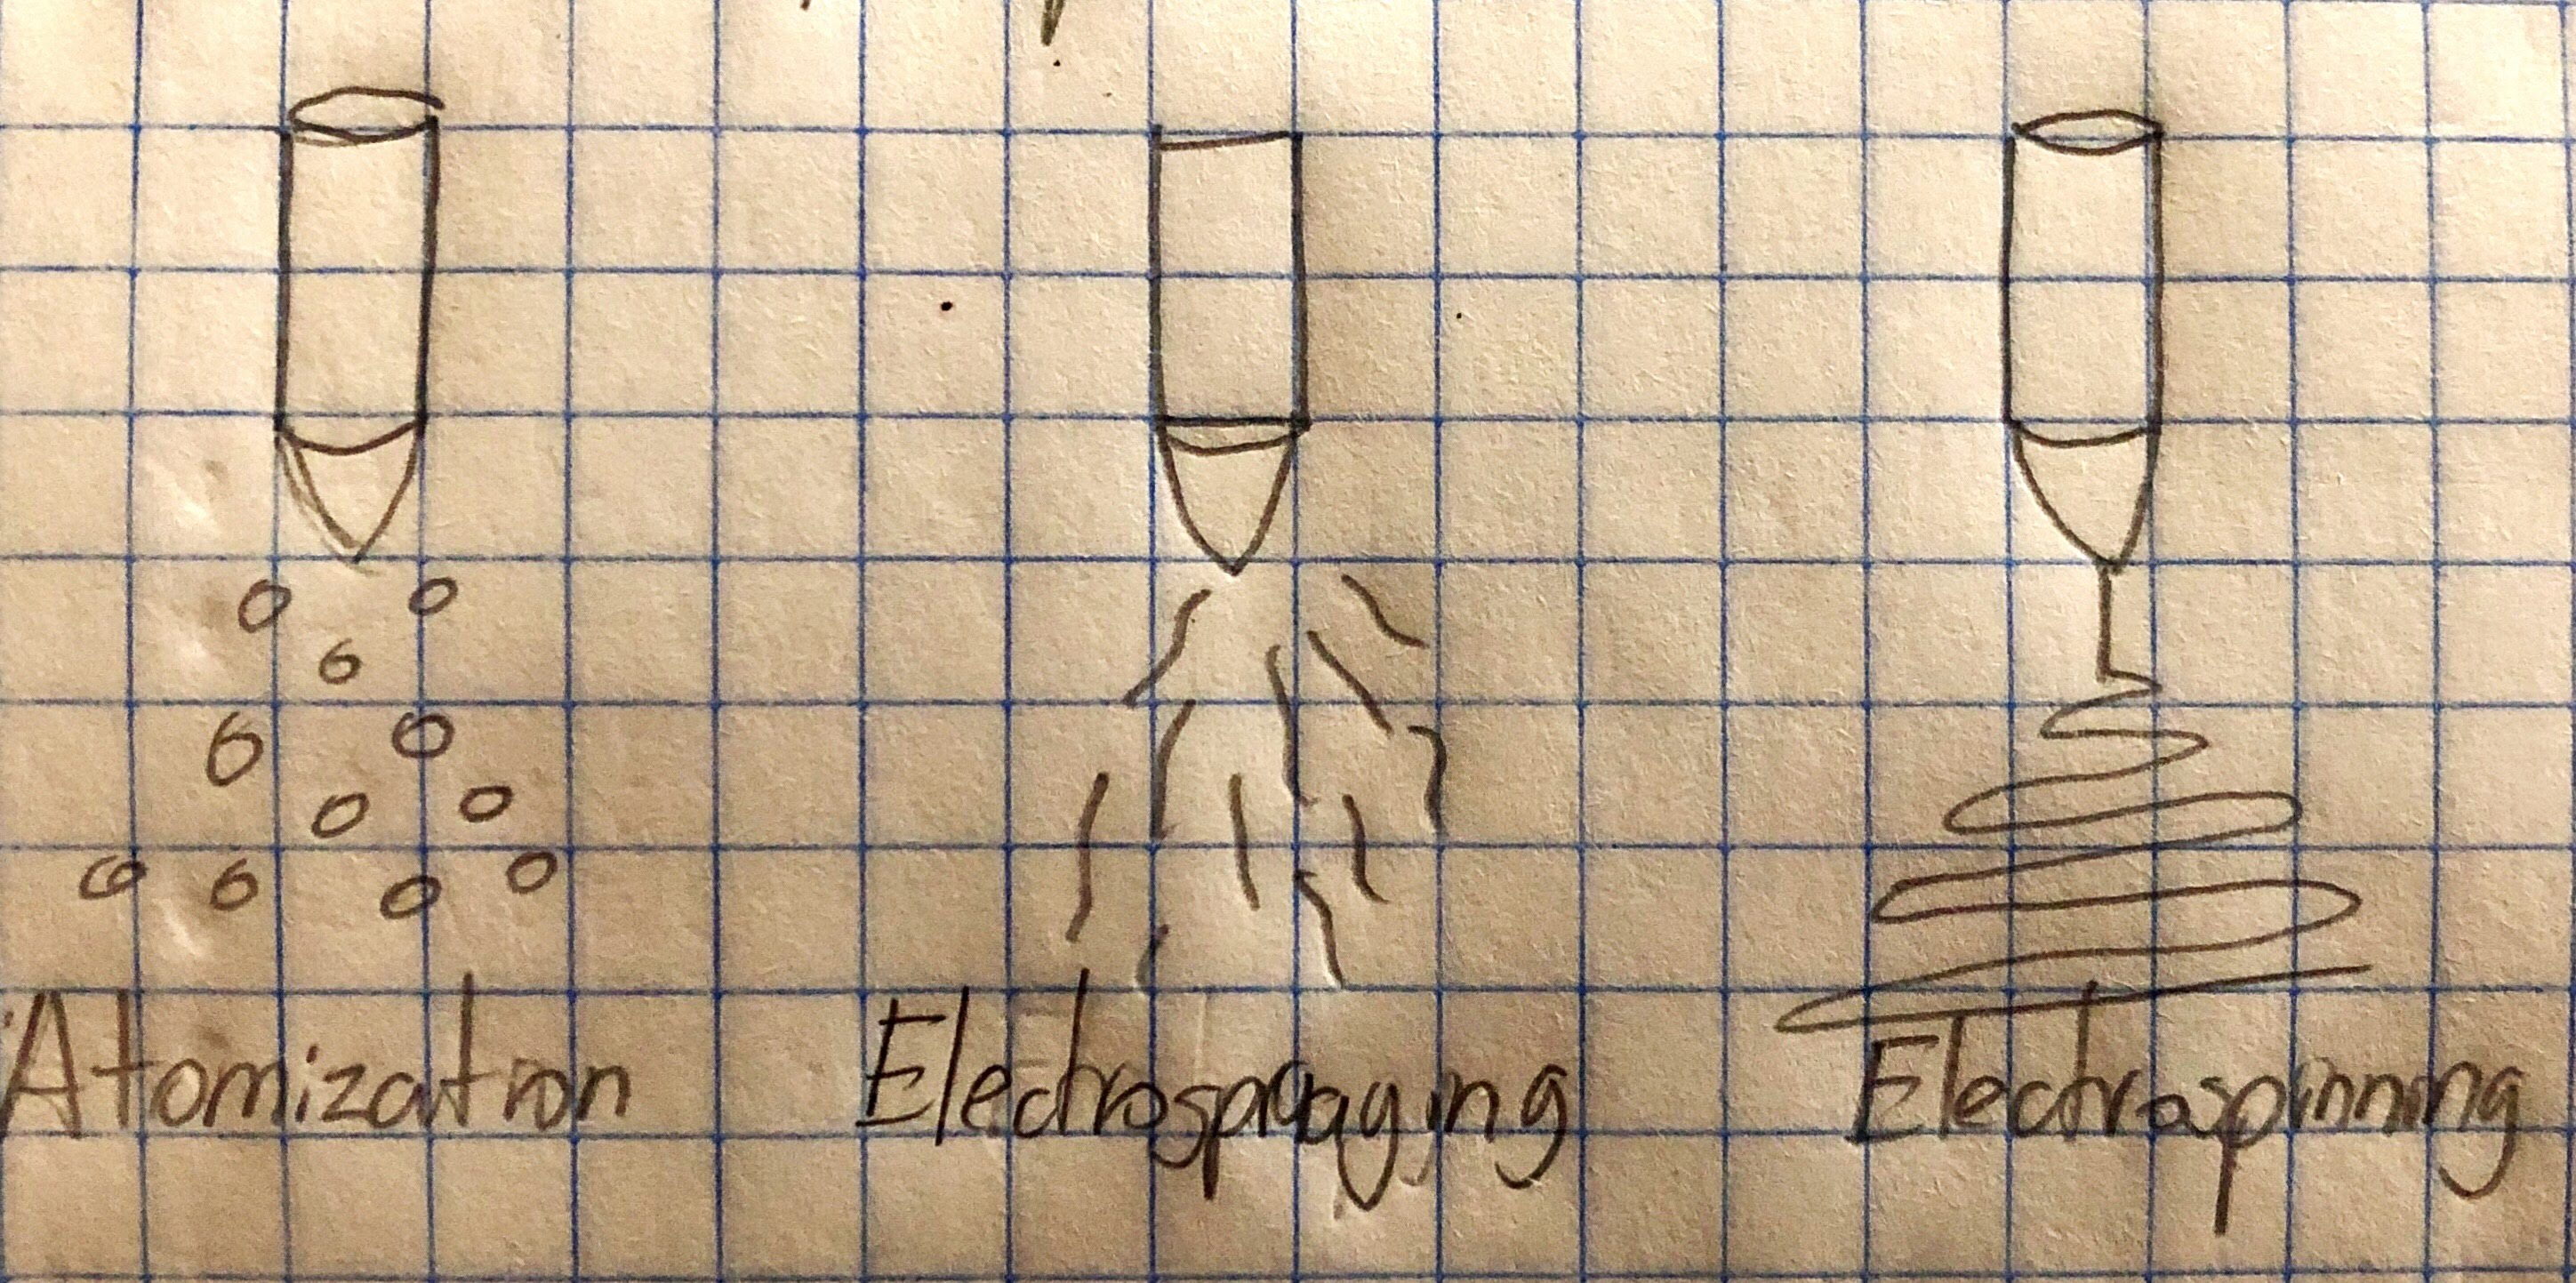
\includegraphics{images/f10bcbc9-719b-4a8d-8a38-930cc6ea2d0f-uimg_ehdprocesses.jpg}}{}
\makeatother 
\caption{{Electrohydro-dynamic techniques}}
\label{f-02e0e3cf88d6}
\end{figure*}
\egroup
In electrospinning the fibers are deposited by an electrical potential difference between the syringe needle and the collector. The supplied polymer (typically a polymer solution) is administrated at a constant rate to create and maintain a polymer drop at the dispensing nozzle. A high voltage (usually DC) is applied between the polymer feed and the collector. As the electric field increases, the polymer drop (held by its surface tension) is then deformed at the tip of the syringe needle to form a conical shape known as Taylor cone. When the electric force overcomes the surface tension force a polymer jet is ejected from the tip of the Taylor cone. As the polymer jet leaves the nozzle, it accelerates and stretches while traveling to the fiber collector. The fiber finally develops with the complete solvent evaporation.





\subsubsection{High voltage power supply: Direct Current \& Alternating Current}Electricity comprises a flow of electrons (negatively charged subatomic particles). In direct current (DC; used for the vast majority ofelectrospinning work) the electrons flow in one direction continually. Itis also possible to have alternating current (AC), which is used to powermost electrical devices in the home. AC involves a periodic change in thedirection of current flow: that is, the electrons first flow in one directionand then switch to flow in the reverse direction. The switch betweendirections is repeated many times per second and is known as the frequency of the AC. Using an AC power supply rather than the conventional DC supply was first shown to generate polymer-based nanofibresin 2004. [3]

The experimental set-up for AC electrospinning is similar to thatfor the DC process, but it does not require a grounded collector. Because the current alternates, the fibres produced at one instant in time carry apositive charge, while those generated shortly thereafter have a negativecharge. The positive and negative fibres thus discharge on each other,which results in an aerogel plume of fibres. The frequency of the AC current determines whether charge carriersof one polarity have sufficient time to charge the solution and result inspinning. The optimal AC frequency is material-dependent and typicallyin the range of 50 Hz{\textendash}1 kHz. [4]

The AC approach has been explored for the fabrication of drugloaded fibres in a few recent studies. In one, Balogh et al. undertook adirect comparison of fibres prepared by DC and AC spinning.5 They usedthe beta-blocker carvedilol as a model drug, and fibres were generatedusing three different polymers: Eudragit EPO, a cationic copolymer soluble below pH 5.0; Eudragit L100-55, an anionic polymer soluble abovepH 5.5; and the neutral polymer poly(vinyl pyrrolidone) (PVP). It wasfound that fibres could be generated with all three polymers from bothtypes of spinning, but that it was possible to use muchfaster flow rates in the AC process. With DC spinning, a maximum flow rate of 5 ml h{\textendash}1 could be achieved, whereas with AC this could beincreased to up to 40 ml h{\textendash}1. All fibres, from both processes and madefrom all polymers, existed as amorphous solid dispersions. The drugrelease profiles were studied, and the AC and DC fibres were found to beindistinguishable in their performance. [Adapted with permission from Balogh, A.; Cselko, R.; Demuth,B.; Verreck, G.; Mensch, J.; Marosi, G.; Nagy, Z. K. `Alternating currentelectrospinning for preparation of fibrous drug delivery systems.' Int.J. Pharm. 495 (2015): 75{\textendash}80. Copyright Elsevier 2015.]

The same team have also compared AC and DC electrospinningof blends of hydroxypropylmethylcellulose (HPMC) and poly(ethyleneoxide) (PEO) with the poorly water-soluble diuretic spironolactone. [6] Both HPMC and PEO alone could be processed by the DC approach. Incontrast, AC electrospinning of HPMC led to a mixture of droplets andfibres, and high-molecular-weight PEOs did not yield any solid productsat all in the AC method. Selecting appropriate blends of the two polymers,however, permitted high-quality fibres to be formed via AC spinning.

AC processing of HPMC or PEO with spironolactone also proved tobe problematic, but again with the right mix of HPMC and PEO drugloaded fibres could be generated. These were able to accelerate thedissolution rate of the drug, even at loadings of up to 40\% w/w. The ACgenerated fibres were found to be several orders of magnitude thinnerthan the DC electrospun fibres despite the flow rate being three timesfaster in the AC process.

Similar observations have been reported using HPMC acetate succinate (HPMCAS) and spironolactone. [7] HPMCAS could not be processedby either DC or AC electrospinning; the addition of PEO permitted fibresto be produced with the DC approach, but not using AC, and the additionof an ionic surfactant or salt was required to produce high-quality fibreswith AC spinning. As with HPMC, the HPMCAS fibres led to a significantenhancement in the dissolution rate

It is thus clear that AC electrospinning is similarly effective to theDC approach in producing drug delivery systems. Although its use in thisregard is in its infancy, given the fact it allows higher throughput than theDC technique, it seems certain that this is an approach which is likely toreceive much more attention in the coming years.



\subsubsection{Polymer reservoir: Polymer melt \& Polymer solution}Another variant of electrospinning which has attracted some attentionin the drug delivery sphere is the melt process. This is discussed indetail in a recent review. [8] In brief, the process is analogous to the solution electrospinning discussed in previous sections, but in place of a polymer solution a melt is used. This adds some complexity to the process, because the syringe and spinneret must be heated to maintain thepolymer in its liquid state. Further, the elevated temperature can potentially lead to drug degradation, since many drugs are thermally labile.The fibres produced in melt spinning are typically found to have largerdiameters than those from the solution route due to the significantlyhigher viscosity of a polymer melt than its solution form. The apparatusused is depicted in [TODO: draw an apparatus used for melt electrospinning].

Despite these apparent disadvantages, there are a number ofattractive aspects of the melt spinning process, not least the fact that itobviates the need to handle large volumes of volatile solvents. This bothrenders the process safer, particularly if it is to be performed on the largerscale, and precludes any solvent contamination in the products.

The first report of a melt electrospun drug delivery system camefrom Nagy and co-workers, who prepared melt-spun fibres of Eudragit EPO loaded with carvedilol. [9] The drug and polymer were melted andmixed to form a homogeneous solid mixture prior to spinning, and thenprocessed as in a solution experiment but with both the syringe and spinneret heated. The melt fibres were much wider than analogous systemsprocessed through solution spinning, with those from melt processinghaving diameters of 5{\textendash}30 \ensuremath{\mu}m, as compared to 300{\textendash}1000 nm for the solution-spun fibres. The drug was completely amorphouslydispersed in the fibers regardless of the processing route. This is asexpected for solution spinning, and in the melt case was thought tobe because the experiment was carried out above the melting point ofcarvedilol. The melt fibres freed their drug loading faster than the solution-spun analogues, despite the much larger surface area of the latter.The authors ascribed this to the fact that the melt fibres had a loose nonwoven structure, whereas those prepared by solution spinning weremore tightly packed.

This work has been built on to blend plasticisers with the polymerEudragit E and carvedilol active ingredient. [10] The plasticisers triacetin,Tween 80 and polyethylene glycol were all investigated with the goal ofreducing the melting point of the polymer/drug blend and thereby permitting lower temperatures to be used for spinning. This should reducethe likelihood of any degradation occurring. High-performance liquidchromatography data obtained on dissolved fibres revealed that the addition of plasticisers clearly reduced the amounts of carvedilol degradation products present after melt spinning

A direct comparison of poly(\ensuremath{\varepsilon }-caprolactone) (PCL) fibres generatedby the melt and solution-spinning approaches has been reported by Lianand Meng. [11] These authors prepared curcumin-loaded fibres of around4 \ensuremath{\mu}m in diameter using both techniques. They found that there was agreater tendency for the curcumin to crystallise using the solution route(a result of its low solubility in the solvent used for spinning). The meltfibres led to a reduced burst release and a slower release rate. Thesefindings were attributed to the solution-spun fibres having a porous structure, which permitted both water ingress and the incorporated curcuminto diffuse out of the polymer matrix

Melt electrospinning typically generates micron-size fibres. In arecent effort, however, highly uniform and precise deposition of PCLnanofibres (817 \ensuremath{\pm} 165 nm) was achieved using a method known as meltelectrospinning writing. [12] This combines melt electrospinning with additive manufacturing (three-dimensional (3D) printing) technology, usinga computer-controlled extruder moving on a translational stage to build a3D structure layer by layer. The 3D fibrous architecture produced allowedefficient in vitro proliferation of primary human mesenchymal stromalcells. The melt electrospinning writing technology can produce regular3D morphologies in a highly controllable and reproducible fashion, andis currently being explored for a range of tissue-engineering applications.

Although melt electrospinning has received much less researchinterest than the solution process, it appears to be equally as flexible interms of handling multiple fluids, and coaxial melt spinning has beenreported. [13] The initial melt spinning experiment is perhaps harder toestablish than the solution route, but it is clear that this approach has agreat deal of unexplored potential in the development of drug deliverysystems.



\subsubsection{Stretching forces}



\paragraph{Centrifugal force}Centrifugal spinning employs a rotating polymer source to generate fibres.Several centrifugal methods can generate nanofibres. These includeForcespinning, which employs rotary speed of above 2000 revolutionsper minute (rpm), [14] electrocentrifugal spinning, [15] which combines astrong electric potential (as in electrospinning) with centrifugal force,and pressurised gyration, which adds high pressure ({\textgreater} 10 kPa) to centrifugal spinning to enhance fibre formation (see section 6.8). [16]

These approaches can be applied to polymer solutions andemulsions, and if the source can be heated also to a polymer melt [TODO: draw an apparatus used for centrifugalspinning]. [17] This technique has received some attention in the contextof drug delivery. For instance, Zander prepared PCL fibres using both thesolution and melt variants of the centrifugal technique. [18] This authoremployed spinning speeds in the range of 3000{\textendash}18,000 rpm, yieldingfibres of 10 \ensuremath{\mu }m in diameter. PC12 neuron cells could be successfullygrown on the fibres, demonstrating that they have potential in nervetissue engineering.

In other work, centrifugally spun PCL/PVP fibres containing theantibiotic tetracycline have been produced from a methanol/chloroformsolution at 2000 rpm. [19] These were sub-micron in their diameters, andhighly aligned. The rate of drug release could be tuned by varying thePCL/PVP ratio in the fibres, and the fibres were found to be effective ininhibiting bacterial growth. Core/shell fibres for the delivery of growthfactors have further been reported from centrifugal spinning of a waterin-oil emulsion, with PCL dissolved in the oil phase. [20]

Fibres have also been made using a melt process with sucrose (asugar dimer) loaded with a range of poorly water-soluble drugs, includingolanzapine (an antipsychotic medicine) and piroxicam (a non-steroidalanti-inflammatory). [21] The fibres were 10{\textendash}15 \ensuremath{\mu }m in diameter, and the dissolution rate of the drugs enhanced after fibre formation.

Since the centrifugal spinning approach is a simple one whichallows relatively large-scale production of fibres, [22] it appears to havemuch promise in the drug delivery field. It can also be coupled toelectrospinning, with both centrifugal and electrical forces applied simultaneously to drive solvent evaporation. [15] Such centrifugalelectrospinning uses the same equipment as the standard centrifugalprocess but additionally applies a high voltage between the rotatingspinneret and the collector. It has been reported to lead to significantlyhigher throughput than standard electrospinning, [23] and to producehighly aligned fibres. [23, 24] Centrifugal electrospinning has further beendemonstrated to have potential in the production of drug deliverysystems, with a recent report of PVP fibres loaded with the antibiotictetracycline hydrochloride. [25] Production rates of up to 120 g h{\textendash}1 couldbe realised.



\paragraph{Blowing forces}A pressurised gas can be exploited to produce nanoscale fibres, startingeither with a polymer solution in a technique known as solution blowingor from a molten polymer source (melt blowing). The experimentalapparatus used is similar to electrospinning, in that a polymer solution(or melt) is expelled through a needle (spinneret) at a controlled rate.The spinneret is surrounded by an outer nozzle which applies pressuredgas to the fluid being expelled, as illustrated in [TODO: draw an apparatus used for solution blow spinning or melt blowing]. [26]

A few studies have explored solution blowing in drug delivery,with the first such work being from Oliveira et al. in 2013. [27] These authors prepared poly(lactic acid) (PLA) fibres loaded with the hormone progesterone, which can be used to regulate the reproductivecycle in livestock. Fibres were produced from solutions with 6\% w/vPLA and between 0 and 8\% w/v progesterone. The PLAis semi-crystalline both before and after processing, while the drug isamorphous post-spinning. The fibres behave very similarly in termsof their release behaviour, regardless of the amount of drug loaded.

A study comparing electrospun and solution-blown fibres of poly(3-hydroxybutyrate-co-3-hydroxyvalerate) loaded with sodium diclofenachas also been reported. [26] The drug-loaded fibres were slightly larger indiameter when generated by electrospinning, and the size uniformitywas higher through solution blowing. In general there was a greateramount of burst release seen with the electrospun fibres, but otherwisethere were no clear trends in the drug release data.

Solution-blown fibres have additionally been created loaded withoil extracted from the medicinal plant Copaifera sp., which is oftenexplored for antimicrobial purposes. [28] These materials were constructedfrom a blend of the polymers PLA and PVP, and were around 1 \ensuremath{\mu}m indiameter. An increased PVP content was found to result in increased antibacterial activity after 24 h.

The melt blowing process has also received some attention in thepharmaceutical setting, and the fibres produced compared with thosefrom both solution and melt electrospinning. [29] Marosi's team generatedformulations from a vinylpyrrolidone{\textendash}vinyl acetate copolymer, employingpoly(ethylene glycol) (PEG) as a plasticiser and carvedilol as a modeldrug. All three methods led to fibres, with the solution electrospun fibresnarrowest (at 2 \ensuremath{\mu}m in diameter), followed by the melt-blown (10\ensuremath{\mu}m) and melt-spun (50 \ensuremath{\mu}m) products. Carvedilol was rendered into the amorphous physical form by all three processing techniques, and all theformulations were able to accelerate the drug dissolution process. Themelt-blown and melt electrospun systems led to the fastest release, withalmost identical release profiles, while the solution-electrospun fibresfreed their drug cargo somewhat more slowly.

A variant of the solution-blowing technique has been applied tothe processing of living cells (in this setting it has been referred to asbiothreading). [30] Using a pressurised coaxial needle with the exteriorfluid comprising a viscous polydimethylsiloxane solution and an aqueouscell suspension in the core, cells can be processed into scaffolds with nonoticeable loss in viability.

Electrospinning and melt/solution blowing can be combined in a processknown as electroblowing. This employs both electricity and a gas flow toaid fibre elongation and solidification. The experimental apparatus usesa similar spinneret to that in [Figure apparatus used for solution blow spinning or melt blowing], and in addition to the gas flowa potential difference is applied between the spinneret and the collector.This technique has been shown to have significant potential in medicalapplications: in 2014, Jiang et al. applied electroblowing in vitro and invivo to deliver a homogeneous and continuous layer of a medical glue tostop bleeding during liver resection. [31]

More recently, Balogh et al. prepared fibres of 2-hydroxypropyl-\ensuremath{\beta }-cyclodextrin loaded with sodium diclofenac. [32] They found that whenelectrospinning this system, very frequent clogging of the spinneretoccurred. Electroblowing overcame this issue and additionally allowedfaster flow rates to be used, increasing the amount of material thatcould be produced. However, the uniformity of the fibre products wascompromised, with more `beads-on-string' type morphology seen withthe blown products. In both cases, the fibres comprised amorphous soliddispersions with no crystalline drug evident. The electroblown fibresdissolved a little more slowly than those from electrospinning, but stillmuch more rapidly than a physical mixture of drug and cyclodextrin.

A subsequent study using Eudragit E and itraconazole (anantifungal active pharmaceutical ingredient) also found that a fasterflow rate could be used in blowing, but that the fibre products from thelatter had less regular morphologies. [33] Again, the drug was amorphouslydispersed in the fibres, and the dissolution profiles of the electrospun andelectroblown systems were very similar.



\paragraph{Electric force}



\paragraph{Microfluidic forces}Microfluidic spinning is based on the use of micro (sub-millimetre)channels. A large number of these are located in a single microfluidicchip, and the rate and time of liquid expulsion from each channel are precisely controlled by computer. Microfluidic spinning can be coupled withelectrospinning, as described in detail in a recent review by Cheng et al. [51]While the productivity of microfluidic methods is a major challenge inscale-up, the technique offers the ability to generate fibres with a highlevel of complexity not easily achievable by electrospinning. For example,using a digitally programmed microfluidic flow, Kang et al. created functional microfibres with continuous spatiotemporal coding along thelength of the fibre. [52] The fibres contained varied chemical compositionsand topography, and localised bioactive agents.

Microfluidic spinning therefore has the potential to enable veryprecisely tuneable loading of different drugs into a single fibre, allowingfor programmable release in different parts of the body at differenttimes. The technique is beginning to be explored for drug deliveryapplications. However, the materials used in microfluidics are usuallyhydrogels (crosslinked polymer networks solvated with water). Theseoften have fast degradation rates and as a result can be unsuitable forthe extended release of drugs, particularly small molecules. To helpmitigate this problem, Chae et al. developed a microfluidic spinningmethod using an isopropyl alcohol sheath flow with an aqueousalginate core flow. [53] This innovation resulted in nanofibres made ofhighly ordered alginate molecules. Ahn et al. loaded ampicillin intoalginate fibres prepared in this manner, [54 and found that the orderedstructure delayed fibre degradation, allowing extended-release profileof ampicillin over 7 days.



\paragraph{Mechanical force}



\subsubsection{Dispensing nozzle: Coaxial / Monoaxial: Single nozzle / Multinozzle}



\subsubsection{Nozzle-to-substrate distance}



\paragraph{Near Field Spinning}Figure~\ref{f-fe28447572e9} describes a typical near-field electrospinning set-up \unskip~\cite{527120:12073538}. Two sub-techniques can be derived from electrospinning depending on the distance between the dispensing electrode and the collector. The process in which the electrospun jet can be controlled near the tip is called NFES or near-field electrospinning \unskip~\cite{527120:12033655}. Moreover, if the distance between the collector and the dispensing needle is greater, the configuration is known as FFES or far-field electrospinning \unskip~\cite{527120:12073581}.



\paragraph{Far Field Spinning}In  a far field electrospinning the process continues ... Decreasing the jet diameter, the surface charge density increases and the resulting high repulsive forces split the jet into several smaller jets. The jet is seriously elongated by a bending and whipping processes caused by electrostatic repulsion initiated at small bends in the fiber, until it is finally deposited on the collector. Two types of collector may be used, either stationary or rotary collector.
    
\section{"Electro - DC - monoaxial - solution - NF - spinning"}

\bgroup
\fixFloatSize{images/397f8131-9380-45a0-8289-a666e0d4f8c6-udrf_nfes.jpg}
\begin{figure*}[!htbp]
\centering \makeatletter\IfFileExists{images/397f8131-9380-45a0-8289-a666e0d4f8c6-udrf_nfes.jpg}{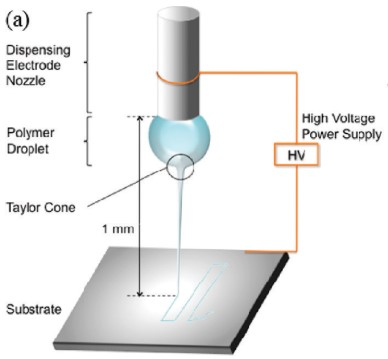
\includegraphics{images/397f8131-9380-45a0-8289-a666e0d4f8c6-udrf_nfes.jpg}}{}
\makeatother 
\caption{{Typical near-field electrospinning set-up \unskip~\protect\cite{527120:11973130} .}}
\label{f-fe28447572e9}
\end{figure*}
\egroup
Near-field electrospinning is considered to be an outstanding technique to fabricate polymer fibers with spatial control and it has suffered several modifications to improve the precision and accuracy of the fiber deposition. This paper intents to collect the NFES variants of electrospunable polymer solutions with spatial control in recent research.
    
\section{Polymer Solution}
In electrospinning, it is typically agreed that the diameter of the fibers increased with higher concentration due to greater viscosity which withstands stretching. In near field electrospinning, similar observations have been reported where concentration increases, fiber diameter increased\unskip~\cite{527120:11974306,527120:11974329}. However, in separate studies by Pan et al.\unskip~\cite{527120:11974317,527120:12321129} using poly(\ensuremath{\gamma }-benzyl \ensuremath{\alpha }, l-glutamate) and polyvinylidene fluoride (PVDF) reported reduction in fiber diameter with increasing concentration.
\begin{table*}[!htbp]
\caption{{Approximation process to estimate the critical polymer concentration. Several polymer concentrations are tried and the resulting jets are observed until a continuous stream is achieved.} }
\label{tw-8687dd17082c}
\def\arraystretch{1}
\ignorespaces 
\centering 
\begin{tabulary}{\linewidth}{LL}
\tbltoprule Observation & Concentration Adjustement\\
\tblmidrule 
Dripping, no stream &
  Increase\\
Splitting small droplets &
  Increase slightly\\
Steady stream &
  No concentration adjustment\\
Splitting large globs &
  Decrease slightly\\
Nozzle clogging  &
  Decrease\\
\tblbottomrule 
\end{tabulary}\par 
\end{table*}




\subsection{Polymers}The polymer selection is in function on the intended application. For example, a fast dissolving hydrophilic polymer such as poly(ethylene oxide) (PEO) is used for fast drug delivery systems. Otherwise, slow dissolving polymers such as poly($\varepsilon $-caprolactone) (PCL) or poly(lactic-co-glycolic acid) (PLGA) are implemented. \unskip~\cite{527120:13082763}

The polymer molecular weight along with the polymer concentration and solvent selection have a direct effect on the solution viscosity, conductivity and surface tension, hence the solution behavior in the electrospinning process. The spunable viscosity range varies with the polymer and solvent. 

Solutions with low viscosity are prone to insufficient polymer chain entanglements to produce fibers.\unskip~\cite{527120:13082763} On the other hand, if the solution is too viscous, then the surface tension cannot easily be overcome by the electric field. In both cases, the result can be droplets or particles forming rather than fibers; see Table~\ref{tw-8687dd17082c}.



\subsection{Solvents}The solvent used must be capable of dissolving the polymer of interest at an appropriate concentration to form fibers, and must posses a suitable volatility. A low-volatility solvent like water may fail to evaporate completely over the distance between the spinneret and the collector. When the fibers form, they will hence contain residual water owing to this incomplete evaporation. The residue solvent will subsequently evaporate from the fibers upon storage, resulting in ribbon-like (flattened) fibers, wrinkles on the fiber surface or fused fibers. On the other hand, a high-volatility solvent may evaporate very quickly, leading to larger fiber diameters (less time for elongation before solidification) and clogging of the spinneret (due to drying of the liquid at the spinneret before jetting, or drying of the Taylor cone during jetting). Solvents commonly used for electrospinning include ethanol, chloroform, dichloromethane and hexafluoroisopropanol.

Mixtures of miscible solvents can be used to ensure that sufficient polymer can be dissolved to give a solution of appropriate viscosity and volatility with suitable dielectric constant range to allow fiber formation. However, care must be taken because using a mixture of solvents with very different volatilities can result in porous fiber structures, as reported by Katsogiannis et al. for organic solvent mixtures with dimethyl sulfoxide (DMSO).\unskip~\cite{527120:13082766} DMSO evaporates much more slowly than the organic solvents used, which results in its incorporation into the fibers. The DMSO will eventually evaporate, yielding porous fibers.

It is also important to take into account the surface tension of the solution. Solvents with very high surface tensions (e.g. water) can result in instability arising during the spinning process, and a broad range of fiber diameters in the products. If necessary, a surfactant can be added to reduce the surface tension, but this will be incorporated into the fibers produced.
    
\section{Effect of the NFES Parameters}

\bgroup
\fixFloatSize{images/d29b646e-eca6-4b31-ab15-4cfc6fc94809-udrf_electrospinningvariants.jpg}
\begin{figure*}[!htbp]
\centering \makeatletter\IfFileExists{images/d29b646e-eca6-4b31-ab15-4cfc6fc94809-udrf_electrospinningvariants.jpg}{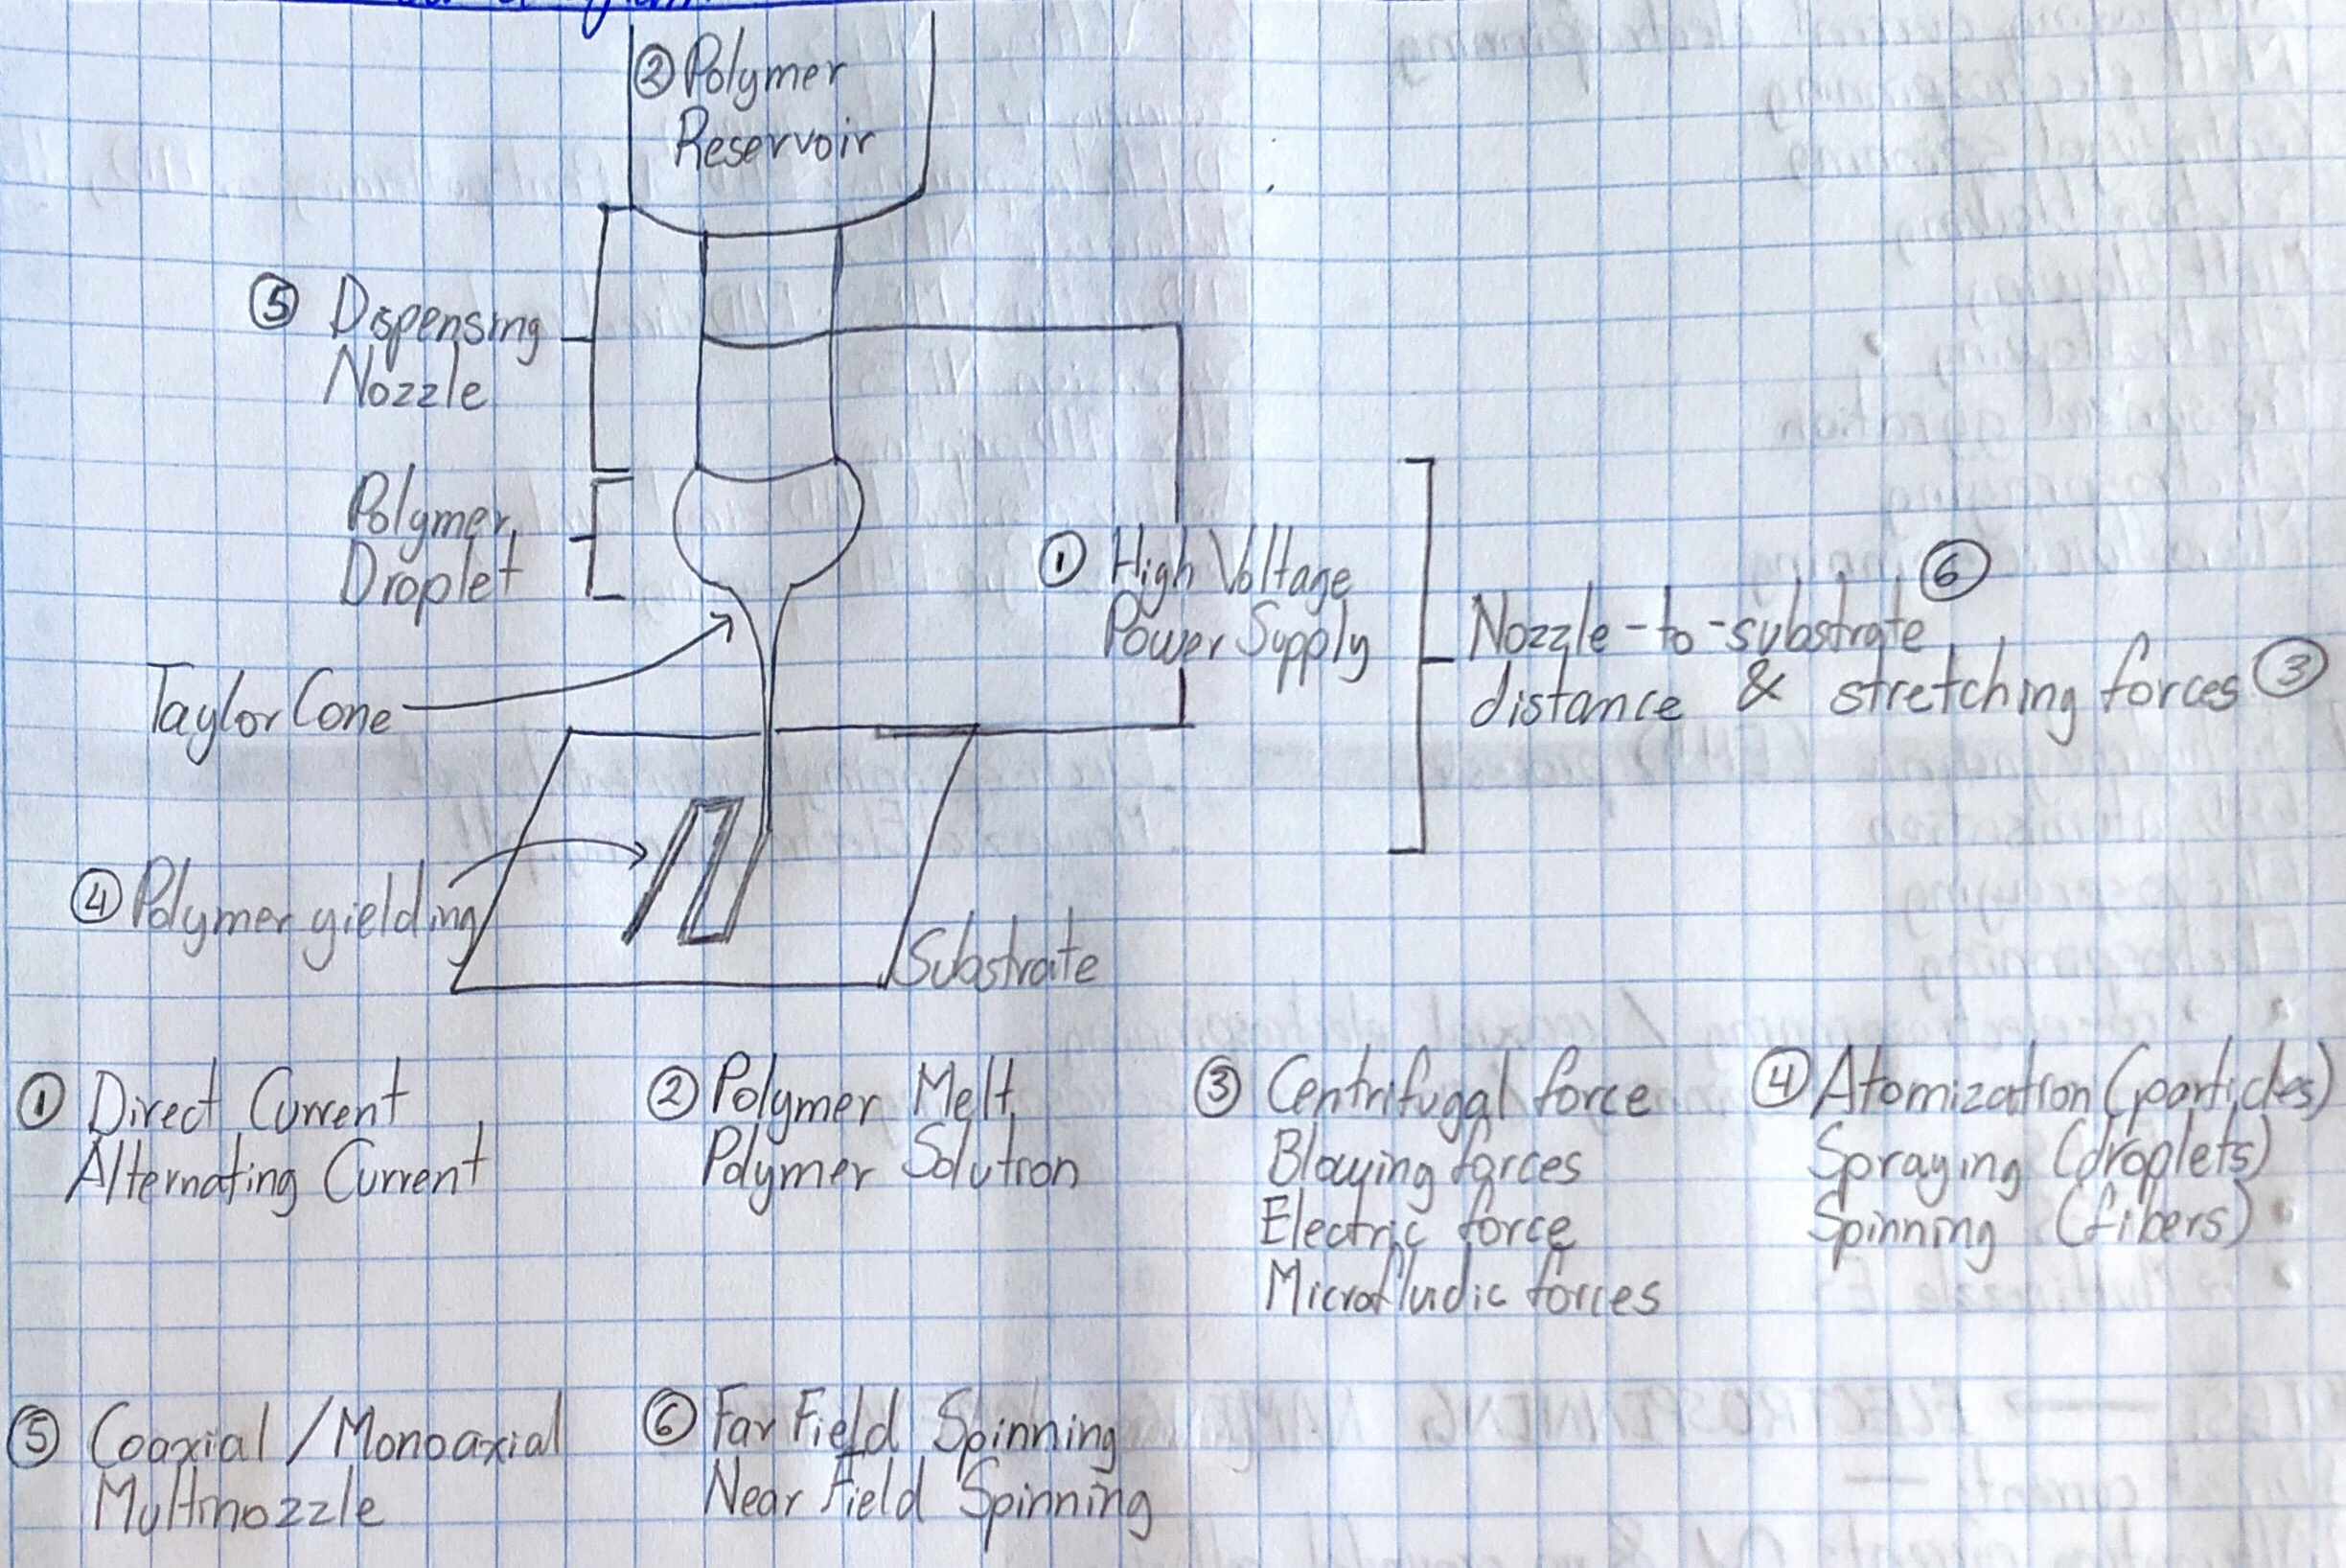
\includegraphics{images/d29b646e-eca6-4b31-ab15-4cfc6fc94809-udrf_electrospinningvariants.jpg}}{}
\makeatother 
\caption{{Near-Field ES Process Parameters}}
\label{f-3629d3a3f9cf}
\end{figure*}
\egroup
To spin nano fibers at close distances, the initial diameter of the jet is required to be as small as possible since stretching of the thread is limited. Kameoka et al.\unskip~\cite{527120:12321556} demonstrated that a small initial spinning radius can be achieved using an atomic force microscope tip with a small polymer solution drop at the tip.

Near-field electrospinning, has exhibited to be capable fabricate nano fibers over and nano fiber patterns \unskip~\cite{527120:11974321}. Nevertheless, having a small polymer solution drop at the nozzle tip limits the length of the fibers that can be fabricated in a continuous manner. Using a spinneret with a reservoir (e.g. syringe) of solution generally produces fibers with diameter of a few micrometers \unskip~\cite{527120:11974310,527120:11974326}, since it creates a limit to which the nozzle inner diameter can be reduced to allow the solution to flow through.

Coppola et al.\unskip~\cite{527120:11974307} have showed a NFES variant that allows polymer nano fibers to be deposited directly from a polymer drop, averting the issue of nozzle clogging. The fibers are also prone soaking after deposition thus giving the fibers a semi-circular cross-section as depicted in Xue et al.'s\unskip~\cite{527120:11974326} work. 



\subsection{Nozzle spinneret}The thinnest nozzles in literature so far are about 100 $\mu m $ in diameter, for instance Chang et al.\unskip~\cite{527120:11974306} used a 100 $\mu m $ inner diameter needle tip to electrospin poly(ethylene oxide) (PEO) and Camillo et al.\unskip~\cite{527120:12322072} used a micro-diameter tip Tungsten spinneret in a 26G needle to electrospin co-polymer, poly[2-methoxy-5-(2-ethylhexyloxy)-1,4-phenylenevinylene] (MEH-PPV) with poly(ethylene oxide) (PEO). The nozzle most commonly comprises a simple narrow-bore, blunt-end metal needle. The diameter of the needle can vary, but most commonly researches work with internal diameters below 1 $mm $ . This translates to needles of gauge 18{\textendash}22. In general, this simple spinneret design can be used to achieve successful spinning. A blunt-end rather than a tapered-end for the needle exit is important as the size distribution of the products increase with an increase in needle tip angle. However, it should be noted that there will be some interactions between the solvent and polymer molecules in the solution and the metal surface of the spinneret. There will exist some attractive forces between the polar groups in the polymer and the electropositive metal surface, which can act counter to the drawing force of the electric field and can pull the polymer solution back into the spinneret. It has been found that coating the spinneret exterior in a non-conductive and non-stick polymer such as Teflon can reduce these interactions.\unskip~\cite{527120:13082768} As a result, the electrical energy can be more efficiently used to elongate and narrow the polymer jet, and narrower fibers can be produced. In addition, strong attractive forces between the polymer jet and the metal spinneret can result in fibers becoming attracted to the needle, leading to lower yields and potentially to blocking of the exit orifice. This effect too can be ameliorated using an epoxy coating.\unskip~\cite{527120:13082811}



\subsection{Applied Voltage}In recent literature, near field electrospinning has been studied to reduce the fiber diameter and to improve the fiber deposition accuracy. Camillo et al.\unskip~\cite{527120:12322072} demonstrated that the application of a modified fine tip nozzle enables the fabrication of 100 $nm $ diameter fiber at a nozzle-to-substrate distance of 500 $\mu m $ and an applied voltage of 1.5 $kV $ . On the other hand, Bisht et al.\unskip~\cite{527120:11973130} and Chang et al.\unskip~\cite{527120:11974306} came to the conclusion higher voltages yield thicker micro-fibers with a loss in jet stability.

This discrepancy in literature between the applied voltage and resulting fiber diameter is due to the relationship with other variables such as nozzle-to-substrate distance and solution deposition rate. For instance, if a high voltage is applied at a low deposition rate then electrospraying is achieved, meaning the formation of several non-continuous fibers. The applied voltage shall be sufficient to break the surface tension and initiate the jet, but low enough to avoid multiple jets at the nozzle tip.

Bisht et al.\unskip~\cite{527120:11973130} achieved the fabrication of thinner fibers with spatial control by reducing the applied voltage to 200-600 $V $  at a nozzle-to-substrate distance of 0.5-1 $mm $. The low voltage setting does not create enough charge to break the polymer solution surface tension to initiate the electrospinning process.

Bisht et al.\unskip~\cite{527120:11973130} and Chang et al.\unskip~\cite{527120:11974306} initiated the electrospun fibers by mechanically pull the polymer solution at the nozzle tip using a micro-probe tip. Chang and coworkers reduced the applied voltage from 1.5 $kV $ to 600 $V $ with a nozzle-to-substrate distance of 500 $\mu m $ to yield a fiber diameter between 3 $\mu m $  and 50 $nm $ . With an applied voltage of 200 $V $ and a nozzle-to-substrate distance of 1 $mm $ , PEO nano fibers were deposited with a diameter about 20 $nm $.

In near-field electrospinning, the applied voltage has an impact on the produced fiber morphology. For instance, a voltage higher or lower to the optimum voltage will translate into an increase in fiber diameter. Song et al.\unskip~\cite{527120:11974320} demonstrated that a decrease in voltage from 400 to 500 $V $ can reduce the fiber diameter from 160 to about 60 $nm $with a nozzle-to-substrate distance of 20 $\mu m $. The optimum voltage is achieved when a balance is attained between the stretching of the jet and the speed at which it hits the substrate. The increase of voltage yields thinner fibers as it causes greater stretching, and a greater jet acceleration.

Another workaround to break the polymer solution surface tension is to initialize the NFES process with a higher voltage and then lower the voltage once the jet is created. Huang et al.\unskip~\cite{527120:11974311} implemented the previous and yield ordered fibers with a distance between adjacent fibers of 50 $\mu m $. In most cases, a positive voltage is applied to the spinneret.



\subsection{Nozzle-to-substrate distance}In NFES, the fiber morphology can be altered by the control of the height between the nozzle and the substrate (collector). With the decrease of the nozzle-to-substrate distance, the electric field strength increases; however it can cause incomplete solvent volatilisation and possible short circuits between the collector and the nozzle tip.

An optimal nozzle-to-substrate distance shall be defined to ensure the fabrication of dry continuous fibers. If the solvent is not well evaporated, the produced fibers are prone to defects; on the other hand if solidification happens too fast, the solids can block the spinneret which can prevent a continuous fiber yield. Furthermore, the polymer jet will discharge itself as soon as possible, therefore long distances can result in low yields.

Typically, metal nozzle tips are used, with small inner diameters. From literature, needles with small diameters produce thinner fibers. A thin nozzle tip can help the reduction of the fiber diameter, but also it is more likely to become blocked.



\subsection{Electric field}Recent literature suggests that the fiber morphology depends on the electric field profile created by the applied voltage during NFES. Since the electric field is an induced force that attracts the solution jet towards the desired location within the collector.

Bisht et al.\unskip~\cite{527120:11973130} and Min et al.\unskip~\cite{527120:11974316} have reported the ability to electrospin nano fibers with high accuracy. Min et al. \unskip~\cite{527120:11974316} implemented a NFES setup with multiple "field-effect transistors" on a flexible polyacrylate collector with an x-y stage velocity of 13.3 $cm/s $ to fabricate fibers with a diameter about 289 $nm $ and a distance between adjacent fibers of 50 $\mu m $. 

On the other hand, Bisht et al.\unskip~\cite{527120:11973130} showed evidence of fabricated fibers with low-voltage NFES with high accuracy and precision. Bisht et al.'s suspended fibers were deposited over carbon posts with a distance between adjacent fibers of 100 $\mu m $ with diameter of 30 $\mu m $\unskip~\cite{527120:11973130}.

The employment of guided electrodes in NFES, adapts the fabrication process to yield a more accurate fiber deposition. For instance, Kim et al.\unskip~\cite{527120:11974313} manufactured ink patterns on a paper with silver nano particles. The printed patterns aid the fibers to land on the desired location. Kim et al.\unskip~\cite{527120:11974313} electrospun the fibers with a distance between adjacent fibers of 150 $\mu m $.

Xu et al.\unskip~\cite{527120:11974325} created a straight jet from the nozzle tip to the substrate using a guiding electrode underneath the collector. The purpose of the guiding electrode is to adjust the path of the NFES jet. With the guiding electrode implementation, the fiber's spread was reduced from 74 $\mu m $ to 7 $\mu m $.



\subsection{Substrate}Due to the close distance between the grounded substrate and the charged spinneret in NFES, the set up is prone to electrical shorts. In NFES, when a short circuit takes place, the electrospinning process is interrupted resulting in the fabrication of discontinuous fibers. Two workarounds to avoid electrical shorts is to lower the applied voltage and to install less conductive substrates \unskip~\cite{527120:11974315,527120:12322289}.

Liu et al.\unskip~\cite{527120:11974315} discovered that the fiber alignment is improved by using a glass-cooper foil substrate, however the well aligned fibers are spoiled after prolonged depositions due to residual charges. Additionally, the effect of residual charges is amplified with the used collector substrate contains a conductive layer and a non-conductive layer\unskip~\cite{527120:11974315}.

On the other hand, Choi et al.\unskip~\cite{527120:12322289} implemented a hydrophobic substrate to deposit the fibers with plasma treatment to increase the conductivity of selected areas. NFES was carried put with precise deposition as the fibers were placed as per the desired design within the hydrophilic substrate.
\begin{landscape}
\makeatletter\@twocolumnfalse\makeatother
\begingroup
\makeatletter\if@twocolumn\@ifundefined{theposttbl}{\gdef\TwoColDocument{true}\onecolumn\onecolumn}{}\fi\makeatother \setlength\LTcapwidth{\textheight}
\begin{longtable}{p{\dimexpr.1641\linewidth-2\tabcolsep}p{\dimexpr.13520000000000005\linewidth-2\tabcolsep}p{\dimexpr.1662\linewidth-2\tabcolsep}p{\dimexpr.46839999999999996\linewidth-2\tabcolsep}p{\dimexpr.0661\linewidth-2\tabcolsep}}
\caption{{Electrospun Polymer Solutions - Solution and Process Parameters} }
\label{tw-bab4042dace7}
\def\arraystretch{1}\\\endfirsthead \hline \noalign{\vskip3pt} \noalign{\textit{Table \thetable\ continued}} \noalign{\vskip3pt} \hline \endhead \hline \noalign{\vskip3pt} \noalign{\textit{\hfill Continued on next page}} \noalign{\vskip3pt} \endfoot \endlastfoot 
\tbltoprule Polymer(s) & Solvent(s) & NFES Variant & Process Parameters and Fiber Characterization & Ref.\\
\tblmidrule 
Poly(ethylene oxide) (PEO; MW = 4,000,000 $g/mol $) &
  Deionized water &
  Low-Voltage NFES (LV NFES) &
  \textbf{Solution Concentration:} 1, 2, and 3 $wt\% $ PEO \mbox{}\protect\newline \textbf{Nozzle:} 27 gauge type 304; stainless steel needle \mbox{}\protect\newline \textbf{Solution deposition rate:} lower than 1$\mu L / h $ \mbox{}\protect\newline \textbf{Nozzle-to-substrate distance:} 1$mm $ \mbox{}\protect\newline \textbf{Substrate composition: }Pyrolyzed SU-8 carbon and Si \mbox{}\protect\newline \textbf{Applied voltage: }polymer jet initiated at 400-600 $V $ and dispensed at 200-400 $V $ \mbox{}\protect\newline \textbf{x-y stage velocity:} 10-40$mm/s $ \mbox{}\protect\newline \textbf{Fiber Diameter:} 50-425$nm $ \mbox{}\protect\newline \textbf{Distance between adjacent fibers:} \textit{Not determined} &
  \unskip~\cite{527120:11973130}\\\cline{1-1}\cline{2-2}\cline{3-3}\cline{4-4}\cline{5-5}
Poly[2-methoxy-5-(2-ethylhexyloxy)-1,4-phenylenevinylene] (MEH-PPV; MW = 380,000 $g/mol $) with Poly(ethylene oxide) (PEO; MW = 300,000 $g/mol $) &
  acetonitrile toluene mixture (65/35); acetic acid toluene (17/83); pure toluene &
  Typical NFES process &
  \textbf{Solution Concentration:} \mbox{}\protect\newline 10$mg $ of MEH-PPV in 2$mL $ of toluene; 500$\mu L $ of MEH-PPV solution with 250$mg $ of PEO in 3.5$mL $ of acetonitrile / toluene (65 / 35); 500$\mu L $ of MEH-PPV solution with 250$mg $ of PEO in 3$mL $ of acetic acid / toluene (17 / 83). The resulting MEH-PPV/PEO concentration is 0.08 $wt\% $ \mbox{}\protect\newline \textbf{Nozzle:} mm-diameter tip Tungsten spinneret in a 26 gauge needle \mbox{}\protect\newline \textbf{Solution deposition rate:} 50$\mu L / h $ \mbox{}\protect\newline \textbf{Nozzle-to-substrate distance:} 500$\mu m $ \mbox{}\protect\newline \textbf{Substrate composition:} SiO2/Si (oxide thickness = 800 nm) \mbox{}\protect\newline \textbf{Applied voltage:} around 1.3$kV $ \mbox{}\protect\newline \textbf{x-y stage velocity:} 50$cm/s $ \mbox{}\protect\newline \textbf{Fiber Diameter:} 100$nm $ \mbox{}\protect\newline \textbf{Distance between adjacent fibers:} around 100$\mu m $ &
  \unskip~\cite{527120:11974305}\\\cline{1-1}\cline{2-2}\cline{3-3}\cline{4-4}\cline{5-5}
Poly(ethylene oxide) (PEO; MV = 300,000 $g/mol $) &
  Water &
  Scanning Tip Electrospinning and NFES &
  \textbf{Solution Concentration:} 7$wt\% $ PEO \mbox{}\protect\newline \textbf{Nozzle:} Needle outer diameter of 200$\mu m $ and inner diameter of 100$\mu m $ \mbox{}\protect\newline \textbf{Solution deposition rate:} 0.1$\mu L / h $ \mbox{}\protect\newline \textbf{Nozzle-to-substrate distance:} 500$\mu m $ \mbox{}\protect\newline \textbf{Substrate composition:} \textit{Not determined} \mbox{}\protect\newline \textbf{Applied voltage:} polymer jet initiated at 1.5 $kV $ and dispensed at 600$V $ \mbox{}\protect\newline \textbf{x-y stage velocity:} 120$mm/s $ \mbox{}\protect\newline \textbf{Fiber Diameter:} 709$\pm $131$nm $; 49-74$nm $ when applied voltage is 800$V $ \mbox{}\protect\newline \textbf{Distance between adjacent fibers:} \textit{ Not determined} \mbox{}\protect\newline \textbf{Notes:} 108$m $ yield in 15$min $ with a fiber diameter of 709$\pm $131$nm $ &
  \unskip~\cite{527120:11974306}\\\cline{1-1}\cline{2-2}\cline{3-3}\cline{4-4}\cline{5-5}
Poly(vinylidine fluorid) (PVDF; MW = 440,000 $g/mol $) &
  N,N Dimethylformamide (DMF) &
  Helix Electrohydro-dynamic Printing (HE-printing) &
  \textbf{Solution Concentration:} 1.8$g $ PVDF in 4.1$g $ of DMF and 4.1$g $ of acetone. The resulting concentration is 18\% PVDF. \mbox{}\protect\newline \textbf{Nozzle:} Needle outer diameter of 510$\mu m $ and inner diameter of 260$\mu m $ \mbox{}\protect\newline \textbf{Solution deposition rate:} 400$nL/min $ \mbox{}\protect\newline \textbf{Nozazle-to-substrate distance:} 10-50$mm $ \mbox{}\protect\newline \textbf{Substrate composition: }Poly(dimethylsiloxane) (PDMS) on Ecoflex \mbox{}\protect\newline \textbf{Applied voltage:} 1.5{\textendash}3$kV $ \mbox{}\protect\newline \textbf{x-y stage velocity:} 0-400$mm/min $ \mbox{}\protect\newline \textbf{Fiber Diameter:} about 1.5-3$\mu m $ \mbox{}\protect\newline \textbf{Distance between adjacent fibers:} \textit{Not determined} &
  \unskip~\cite{527120:11974308}\\\cline{1-1}\cline{2-2}\cline{3-3}\cline{4-4}\cline{5-5}
Polyhedral Oligomeric Silsesquioxane-Poly(Carbonate-Urea)Urethane (POSS-PCU) and Polyhedral Oligomeric Silsesquioxane Poly(Caprolactone-Poly(Carbonate-Urea)Urethane) (POSS-PCL-PCU) \mbox{}\protect\newline (Dry Polycarbonate MW = 2000 $g/mol $) &
  Dimethyl acetamide (DMAC) and 1-Butanol &
  Electrohydro-dynamic 3D Print-patterning or Electrohydro-dynamic Jetting &
  \textbf{Solution Concentration: }POSS-PCU and POSS-PCL-PCU used in 20\%$w/w $ concentration in DMAC \mbox{}\protect\newline \textbf{Nozzle:} needle of 750 $\mu m $ in diameter \mbox{}\protect\newline \textbf{Solution deposition rate:} less than 1$\mu L / min $ \mbox{}\protect\newline \textbf{Nozzle-to-substrate distance: }about between 500$\mu m $ to 2$mm $ \mbox{}\protect\newline \textbf{Substrate composition:} \textit{Not determined} \mbox{}\protect\newline \textbf{Applied voltage:} 8.0-10.0$kV $ \mbox{}\protect\newline \textbf{x-y stage velocity:} 10$mm/s $ \mbox{}\protect\newline \textbf{Fiber Diameter:} 5-50$\mu m $ \mbox{}\protect\newline \textbf{Distance between adjacent fibers: }250$\mu m $ &
  \unskip~\cite{527120:11974310}\\\cline{1-1}\cline{2-2}\cline{3-3}\cline{4-4}\cline{5-5}
Poly(ethylene oxide) (PEO; MW = 300,000 $g/mol $) &
  Distilled water &
  Electrohydro-dynamic Writing or Mechanoelectrospinning (MES) &
  \textbf{Solution Concentration:} 6$wt\% $ PEO \mbox{}\protect\newline \textbf{Nozzle:} \textit{Not determined} \mbox{}\protect\newline \textbf{Solution deposition rate:} 1200$nL/min $ \mbox{}\protect\newline \textbf{Nozzle-to-substrate distance:} 7.5$mm $ \mbox{}\protect\newline \textbf{Substrate composition:} \textit{Not determined} \mbox{}\protect\newline \textbf{Applied voltage:} polymer jet initiated at 2 $kV $ and dispensed at 0.8-1$kV $ \mbox{}\protect\newline \textbf{x-y stage velocity:} around 400$mm/s $ \mbox{}\protect\newline \textbf{Fiber Diameter:} 200-350$nm $ \mbox{}\protect\newline \textbf{Distance between adjacent fibers:} 5$\mu m $ &
  \unskip~\cite{527120:11974311}\\\cline{1-1}\cline{2-2}\cline{3-3}\cline{4-4}\cline{5-5}
Poly(ethylene oxide) (PEO; MW = 300,000 $g/mol $) &
  Deionized water and ethanol with a volume ratio of 3:1 &
  Airflow-assisted Electrohydro-dynamic Direct-writing (EDW) &
  \textbf{Solution Concentration:} 8$wt\% $ PEO \mbox{}\protect\newline \textbf{Nozzle:} Outer airflow passage diameter: 1$mm $ Airflow gas pump pressure: 25$kPa $ Inner liquid passage diameter: 0.21$mm $ \mbox{}\protect\newline \textbf{Solution deposition rate:} 30$\mu L / h $ \mbox{}\protect\newline \textbf{Nozzle-to-substrate distance:} 2$mm $ \mbox{}\protect\newline \textbf{Substrate composition: }Silicon \mbox{}\protect\newline \textbf{Applied voltage:} about 2$kV $ \mbox{}\protect\newline \textbf{x-y stage velocity:} 1-20$mm/s $ \mbox{}\protect\newline \textbf{Fiber Diameter:} 3.73 $\pm $ 1.37$\mu m $ \mbox{}\protect\newline \textbf{Distance between adjacent fibers: }5.13 $\pm $ 6.67$\mu m $ &
  \unskip~\cite{527120:11974312}\\\cline{1-1}\cline{2-2}\cline{3-3}\cline{4-4}\cline{5-5}
Poly(Vinylidene Fluoride) (PVDF; MW = 534,000 $g/mol $) &
  Acetone and Dimethyl Sulfoxide (DMSO) &
  3D Electrospinning &
  \textbf{Solution Concentration:} 17$wt\% $ PVDF; 1.7$g $ of PVDF, 5$g $ of acetone, 0.5$g $ of Capstone FS-66, 5$g $ of DMSO \mbox{}\protect\newline \textbf{Nozzle:} Needle inner diameter of 100$\mu m $ \mbox{}\protect\newline \textbf{Solution deposition rate:} 14$\;nL/min $ \mbox{}\protect\newline \textbf{Nozzle-to-substrate distance:} 750$\mu m $ \mbox{}\protect\newline \textbf{Substrate composition:} A4 size commercial printing paper (Double A) \mbox{}\protect\newline \textbf{Applied voltage:} 1.9$kV $ \mbox{}\protect\newline \textbf{x-y stage velocity:} 10$mm/s $ \mbox{}\protect\newline \textbf{Fiber Diameter:} \textit{Not determined} \mbox{}\protect\newline \textbf{Distance between adjacent fibers:} \textit{Not determined} &
  \unskip~\cite{527120:11974313}\\\cline{1-1}\cline{2-2}\cline{3-3}\cline{4-4}\cline{5-5}
Poly(9-Vinyl Carbazole) (PVK; MW = 1,100,000 $g/mol $) &
  Styrene &
  Typical NFES process &
  \textbf{Solution Concentration:} 3.96$wt\% $ PVK in styrene \mbox{}\protect\newline \textbf{Nozzle:} Needle inner diameter of 100$\mu m $ \mbox{}\protect\newline \textbf{Solution deposition rate:} 500$nL/min $ \mbox{}\protect\newline \textbf{Nozzle-to-substrate distance:} around 2.5$mm $ \mbox{}\protect\newline \textbf{Substrate composition:} Si/SiO2 \mbox{}\protect\newline \textbf{Applied voltage:} 3-4$kV $ \mbox{}\protect\newline x-y stage velocity: 13.3$cm/s $ \mbox{}\protect\newline \textbf{Fiber Diameter:} 289.26 $\pm $ 35.37$nm $ \mbox{}\protect\newline \textbf{Distance between adjacent fibers: }50$\mu m $ \mbox{}\protect\newline \textbf{Notes:} 15$m $ yield in 2$min $ &
  \unskip~\cite{527120:11974316}\\\cline{1-1}\cline{2-2}\cline{3-3}\cline{4-4}\cline{5-5}
Polystyrene (PS; MW \textit{Not determined}) &
  1,2,4-Trichloro benzene &
  Electrohydro-dynamic (EHD) jet printing &
  \textbf{Solution Concentration:} 1 to 5$wt\% $ PS \mbox{}\protect\newline \textbf{Nozzle:} Glass nozzle inner diameter of 2$\mu m $ and outer diameter of 2.66$\mu m $ \mbox{}\protect\newline \textbf{Solution deposition rate:} \textit{Not determined} \mbox{}\protect\newline \textbf{Nozzle-to-substrate distance}: 20, 30, 40$\mu m $ \mbox{}\protect\newline \textbf{Substrate composition: }Si \mbox{}\protect\newline \textbf{Applied voltage:} 500 to 400$V $ in 25$V $ increments \mbox{}\protect\newline \textbf{x-y stage velocity:} 0.01-10$mm/s $ \mbox{}\protect\newline \textbf{Fiber Diameter:} about 60-170$\mu m $ \mbox{}\protect\newline \textbf{Distance between adjacent fibers:} \textit{Not determined} &
  \unskip~\cite{527120:11974320}\\\cline{1-1}\cline{2-2}\cline{3-3}\cline{4-4}\cline{5-5}
Poly(ethylene oxide) (PEO; MW = 300,000 $g/mol $) &
  \textit{Not determined} &
  Typical NFES process &
  \textbf{Solution Concentration:} 3$wt\% $ PEO \mbox{}\protect\newline \textbf{Nozzle:} \textit{Not determined} \mbox{}\protect\newline \textbf{Solution deposition rate:} \textit{Not determined} \mbox{}\protect\newline \textbf{Nozzle-to-substrate distance:} 500$\mu m $ \mbox{}\protect\newline \textbf{Substrate composition:} Si \mbox{}\protect\newline \textbf{Applied voltage:} 1000$V $ \mbox{}\protect\newline \textbf{x-y stage velocity:} 20$cm/s $ \mbox{}\protect\newline \textbf{Fiber Diameter:} 300$nm $ \mbox{}\protect\newline \textbf{Distance between adjacent fibers:} 25$\mu m $ &
  \unskip~\cite{527120:11974321}\\\cline{1-1}\cline{2-2}\cline{3-3}\cline{4-4}\cline{5-5}
Poly(ethylene oxide) (PEO; MW = 2,000,000 $g/mol $) &
  Distilled water &
  Multinozzle NFES &
  \textbf{Solution Concentration:} 5$wt\% $ \mbox{}\protect\newline \textbf{Nozzle:} four-nozzle and six-nozzle array with needle spacing changes from 1.5$mm $ to 3.5$mm $ \mbox{}\protect\newline \textbf{Solution deposition rate:} 1-3$\mu L / min $ \mbox{}\protect\newline \textbf{Nozzle-to-substrate distance:} 2$mm $ \mbox{}\protect\newline \textbf{Substrate composition:} \textit{Not determined} \mbox{}\protect\newline \textbf{Applied voltage:} 1.7-2.7$kV $ \mbox{}\protect\newline \textbf{x-y stage velocity:} \textit{Not determined} \mbox{}\protect\newline \textbf{Fiber Diameter:} 5.47$\mu m $ \mbox{}\protect\newline \textbf{Distance between adjacent fibers:} 3-5 $mm $ &
  \unskip~\cite{527120:11974322}\\\cline{1-1}\cline{2-2}\cline{3-3}\cline{4-4}\cline{5-5}
Poly(ethylene oxide) (PEO; MW = 2,000,000 $g/mol $) &
  Distilled water &
  Multinozzle NFES &
  \textbf{Solution Concentration:}5$wt\% $ \mbox{}\protect\newline \textbf{Nozzle:} Dual-28G-needle array with needle inner diameter of 0.18$mm $ and outer diameter of 0.36$mm $; with needle spacing changes from 2.0$mm $ to 3.0$mm $ \mbox{}\protect\newline \textbf{Solution deposition rate:} 0.2$\mu L / min $ \mbox{}\protect\newline \textbf{Nozzle-to-substrate distance:} 3.0-4.0$mm $ \mbox{}\protect\newline \textbf{Substrate composition: } \textit{Not determined} \mbox{}\protect\newline \textbf{Applied voltage:} 2.0-3.0$kV $ \mbox{}\protect\newline \textbf{x-y stage velocity:} 20$mm/s $ \mbox{}\protect\newline \textbf{Fiber Diameter:} \textit{Not determined} \mbox{}\protect\newline \textbf{Distance between adjacent fibers:} 218-326$\mu m $ &
  \unskip~\cite{527120:11974323}\\\cline{1-1}\cline{2-2}\cline{3-3}\cline{4-4}\cline{5-5}
Poly(ethylene oxide) (PEO; MW = 2,000,000 $g/mol $) &
  Distilled water &
  Multinozzle NFES &
  \textbf{Solution Concentration:}5 $wt\% $ \mbox{}\protect\newline \textbf{Nozzle:} Dual-28G-needle array with needle inner diameter of 180$\mu m $ and outer diameter of 360$\mu m $; with needle spacing changes of 2.0$mm $ \mbox{}\protect\newline \textbf{Solution deposition rate:} 0.2$\mu L / min $ \mbox{}\protect\newline \textbf{Nozzle-to-substrate distance:} 4.0$mm $ \mbox{}\protect\newline \textbf{Substrate composition:} chromium-plated glass \mbox{}\protect\newline \textbf{Applied voltage:} 2.5$kV $ \mbox{}\protect\newline \textbf{x-y stage velocity:} 20$mm/s $ \mbox{}\protect\newline \textbf{Fiber Diameter:} \textit{Not determined} \mbox{}\protect\newline \textbf{Distance between adjacent fibers:} 2.3002-2.7224$mm $ &
  \unskip~\cite{527120:11974324}\\\cline{1-1}\cline{2-2}\cline{3-3}\cline{4-4}\cline{5-5}
Poly(ethylene oxide) (PEO; MW = 4,000,000 $g/mol $) &
  \textit{Not determined} &
  Typical NFES process &
  \textbf{Solution Concentration:} 2$wt\% $ \mbox{}\protect\newline \textbf{Nozzle:} G30 needle with inner diameter of 0.15$mm $ \mbox{}\protect\newline \textbf{Solution deposition rate:} \textit{Not determined} \mbox{}\protect\newline \textbf{Nozzle-to-substrate distance:} 1-3$mm $ \mbox{}\protect\newline \textbf{Substrate composition:} Silicon \mbox{}\protect\newline \textbf{Applied voltage:} 1250$V $ \mbox{}\protect\newline \textbf{x-y stage velocity:} \textit{Not determined} \mbox{}\protect\newline \textbf{Fiber Diameter:} \textit{Not determined} \mbox{}\protect\newline \textbf{Distance between adjacent fibers:} 20$\mu m $ &
  \unskip~\cite{527120:11974325}\\\cline{1-1}\cline{2-2}\cline{3-3}\cline{4-4}\cline{5-5}
Gelatin \mbox{}\protect\newline (porcine skin; MW \textit{Not determined}) &
  Acetic Acid and Ethyl Acetate &
  Typical NFES process &
  \textbf{Solution Concentration:} 11$wt\% $ gelatin, 30$wt\% $ water, 35.4$wt\% $ acetic acid, 23.6$wt\% $ ethyl acetate \mbox{}\protect\newline \textbf{Nozzle:} 19G needle tip with outer diameter of 1.08$mm $ \mbox{}\protect\newline \textbf{Solution deposition rate:} \textit{Not determined} \mbox{}\protect\newline \textbf{Nozzle-to-substrate distance:} 1.25$mm $ \mbox{}\protect\newline \textbf{Substrate composition:} Poly(Dimethylsiloxane) (PDMS) films \mbox{}\protect\newline \textbf{Applied voltage:} 1000$V $ \mbox{}\protect\newline \textbf{x-y stage velocity:} \textit{Not determined} \mbox{}\protect\newline \textbf{Fiber Diameter:} around 2-3$\mu m $ \mbox{}\protect\newline \textbf{Distance between adjacent fibers:} 40$\mu m $ &
  \unskip~\cite{527120:11974326}\\\cline{1-1}\cline{2-2}\cline{3-3}\cline{4-4}\cline{5-5}
Poly(ethylene oxide) (PEO; MW = 300,000 $g/mol $) &
  Water/Ethanol (v/v = 60/40) &
  Typical NFES process &
  \textbf{Solution Concentration:} PEO concentrations of 16\% and 18\% \mbox{}\protect\newline \textbf{Nozzle:} 40$\mu m $ \mbox{}\protect\newline \textbf{Solution deposition rate:} \textit{Not determined} \mbox{}\protect\newline \textbf{Nozzle-to-substrate distance:} 1$mm $ \mbox{}\protect\newline \textbf{Substrate composition:} Planar silicon \mbox{}\protect\newline \textbf{Applied voltage:} 1.7$kV $ \mbox{}\protect\newline \textbf{x-y stage velocity:} 0.36$m/s $ \mbox{}\protect\newline \textbf{Fiber Diameter:} 5.15$\mu m $ \mbox{}\protect\newline \textbf{Distance between adjacent fibers:} \textit{Not determined} &
  \unskip~\cite{527120:11974327}\\\cline{1-1}\cline{2-2}\cline{3-3}\cline{4-4}\cline{5-5}
Poly(ethylene oxide) (PEO; MW = 300,000 $g/mol $) &
  Water/Ethanol (v/v = 3/1) &
  Electrohydro-dynamic Direct-Write (EDW) &
  \textbf{Solution Concentration:} 14$wt\% $ PEO \mbox{}\protect\newline \textbf{Nozzle:} Stainless needle with inner diameter of 210$\mu m $ and outer diameter of 400$\mu m $ \mbox{}\protect\newline \textbf{Solution deposition rate:} 50$\mu L/h $ \mbox{}\protect\newline \textbf{Nozzle-to-substrate distance:} 2$mm $ \mbox{}\protect\newline \textbf{Substrate composition:} Poly(ethylene terephthalate) (PET) \mbox{}\protect\newline \textbf{Applied voltage:} 3$kV $ \mbox{}\protect\newline \textbf{x-y stage velocity:} 700$mm/s $ \mbox{}\protect\newline \textbf{Fiber Diameter:} 15-35$\mu m $ \mbox{}\protect\newline \textbf{Distance between adjacent fibers:} 70$\mu m $ &
  \unskip~\cite{527120:11974328}\\\cline{1-1}\cline{2-2}\cline{3-3}\cline{4-4}\cline{5-5}
Poly(ethylene oxide) (PEO; MW = 300,000 $g/mol $) &
  Deionized water &
  Mechano-Electrospinning &
  \textbf{Solution Concentration:} 3$wt\% $ PEO \mbox{}\protect\newline \textbf{Nozzle:} Stainless steel nozzle with inner diameter of 160$\mu m $ and outer diameter of 310$\mu m $ \mbox{}\protect\newline \textbf{Solution deposition rate:} 50$nL/min $ \mbox{}\protect\newline \textbf{Nozzle-to-substrate distance:} 2-5$mm $ \mbox{}\protect\newline \textbf{Substrate composition:} Silicone \mbox{}\protect\newline \textbf{Applied voltage:}polymer jet initiated at 2$kV $ and dispensed at 1$kV $ \mbox{}\protect\newline \textbf{x-y stage velocity:} 200-400$mm/s $ \mbox{}\protect\newline \textbf{Fiber Diameter:} from 344$\pm $32 to 214$\pm $27$nm $ \mbox{}\protect\newline \textbf{Distance between adjacent fibers:} \textit{Not determined} &
  \unskip~\cite{527120:11974304}\\\cline{1-1}\cline{2-2}\cline{3-3}\cline{4-4}\cline{5-5}
Poly(co-Glycolic) acid (PLGA; MW \textit{Not determined})  &
  Dimethyl Carbonate (DMC) &
  Tethered Pyro-Electrohydro-dynamic Spinning (TPES) &
  \textbf{Solution Concentration:} \textit{Not determined} \mbox{}\protect\newline \textbf{Nozzle:} nozzle-free \mbox{}\protect\newline \textbf{Solution deposition rate:} The drop reservoir is placed directly on a flat substrate \mbox{}\protect\newline \textbf{Nozzle-to-substrate distance:} Taylor's cone is focused and put in direct contact with the collector \mbox{}\protect\newline \textbf{Substrate composition:} Poly(tetrafluoroethylene) (PTFE) coated glass slide \mbox{}\protect\newline \textbf{Applied voltage:} pyro-electric field of between 2.7 $x10^{7}\;V/m $ and 5.5$x10^{7}\;V/m $ \mbox{}\protect\newline \textbf{x-y stage velocity:} \textit{Not determined} \mbox{}\protect\newline \textbf{Fiber Diameter:} 304.7$nm $ \mbox{}\protect\newline \textbf{Distance between adjacent fibers:} \textit{Not determined} &
  \unskip~\cite{527120:11974307}\\\cline{1-1}\cline{2-2}\cline{3-3}\cline{4-4}\cline{5-5}
Poly(ethylene oxide) (PEO; MW = 4,000,000 $g/mol $) with Tetrabutylammonium tetrafluoroborate (TBF; MW \textit{Not determined}) and SU-8 2002 &
  N,N Dimethylformamide (DMF) &
  Typical NFES process &
  \textbf{Solution Concentration:} SU-8/PEO/TBF blend with 0.75$wt\% $ PEO, 1$wt\% $ TBF; the blend is diluted with 30$vol\% $ DMF \mbox{}\protect\newline $\mu m $$\mu m $ \mbox{}\protect\newline \textbf{Solution deposition rate:} \textit{Not determined} \mbox{}\protect\newline \textbf{Nozzle-to-substrate distance:} \textit{Not determined} \mbox{}\protect\newline \textbf{Substrate composition:} Brass disk with a diameter of 38$mm $ \mbox{}\protect\newline \textbf{Applied voltage:} 980$V $ \mbox{}\protect\newline \textbf{x-y stage velocity:} \textit{Not determined} \mbox{}\protect\newline \textbf{Fiber Diameter:} \textit{Not determined} \mbox{}\protect\newline \textbf{Distance between adjacent fibers:} \textit{Not determined} &
  \unskip~\cite{527120:12033655}\\\cline{1-1}\cline{2-2}\cline{3-3}\cline{4-4}\cline{5-5}
Poly(ethylene oxide) (PEO; 200,000 $g/mol $) &
  Water:Ethanol (3:2) &
  Suspension NFES &
  \textbf{Solution Concentration:} 14$wt\% $ PEO \mbox{}\protect\newline \textbf{Nozzle:} stainless steel needle (25 G) with inner diameter of 0.25$mm $ \mbox{}\protect\newline \textbf{Solution deposition rate:} 3$nL/s $ \mbox{}\protect\newline \textbf{Nozzle-to-substrate distance:} between 0.5 and 10$mm $ with 0.5$mm $ increments \mbox{}\protect\newline \textbf{Substrate composition:} Planar silicon electrodes \mbox{}\protect\newline \textbf{Applied voltage:} 1.6$kV $ \mbox{}\protect\newline \textbf{x-y stage velocity:} 50, 150, and 250$mm/s $ \mbox{}\protect\newline \textbf{Fiber Diameter:} 300$nm $ \mbox{}\protect\newline \textbf{Distance between adjacent fibers:} 0.1 and 0.5$mm $ &
  \unskip~\cite{527120:12033656}\\\cline{1-1}\cline{2-2}\cline{3-3}\cline{4-4}\cline{5-5}
Poly(ethylene oxide) (PEO; MW = 400,000 $g/mol $) &
  Deionized water &
  Typical NFES process &
  \textbf{Solution Concentration:} 10$wt\% $ PEO \mbox{}\protect\newline \textbf{Nozzle:} 32G metal needle \mbox{}\protect\newline \textbf{Solution deposition rate:} (Jet impact speed of 5$mm/s $ ) \mbox{}\protect\newline \textbf{Nozzle-to-substrate distance:} 0.5$mm $ \mbox{}\protect\newline \textbf{Substrate composition:} p-type silicon wafer \mbox{}\protect\newline \textbf{Applied voltage:} 400$V $ \mbox{}\protect\newline \textbf{x-y stage velocity:} 5$mm/s $ \mbox{}\protect\newline \textbf{Fiber Diameter:} \textit{Not determined} \mbox{}\protect\newline \textbf{Distance between adjacent fibers:} 50$\mu m $ &
  \unskip~\cite{527120:12033657}\\
\tblbottomrule 
\end{longtable}
\endgroup
\makeatletter\@ifundefined{TwoColDocument}{}{\twocolumn}\makeatother 
\end{landscape}

    
\section{NFES Variants}
[SECTION to be REMOVED]

Nanofibers are fibers with diameters in the nanometer range. The development of nanofibers has greatly enhanced the scope for meeting up the modern world challenges. 

Currently there are two types of electrospinning systems available for producing nanofiber: needle based electrospinning and needleless electrospinning. This paper summarizes the basic mechanism of various types of needle based and needleless spinning systems described in various literatures by many researchers.



\subsection{Low-Voltage NFES (LV NFES) \unskip~\protect\cite{527120:11973130}}Some differences have been discovered between LV-NFES and conventional NFES. Low voltage near field electrospinning produces thinner fibers with lower voltages. Moreover, when implementing a moving stage, the fibers are affected by the mechanical stretching. Bisht et al. \unskip~\cite{527120:11973130} reported that thinner diameters are yield with the increase of the x-y stage velocity, and larger diameters by decreasing the stage velocity.



\subsection{Scanning Tip Electrospinning \unskip~\protect\cite{527120:11974306}}Lorem ipsum dolor sit amet, consectetur adipiscing elit, sed do eiusmod tempor incididunt ut labore et dolore magna aliqua.



\subsection{3D Electrospinning \unskip~\protect\cite{527120:11974313} \mbox{}\protect\newline Electrohydro-dynamic 3D Print-patterning or Electrohydro-dynamic Jetting \unskip~\protect\cite{527120:11974310}}Lorem ipsum dolor sit amet, consectetur adipiscing elit, sed do eiusmod tempor incididunt ut labore et dolore magna aliqua.



\subsection{Multinozzle NFES \unskip~\protect\cite{527120:11974322,527120:11974323,527120:11974324}}Lorem ipsum dolor sit amet, consectetur adipiscing elit, sed do eiusmod tempor incididunt ut labore et dolore magna aliqua.



\subsection{Electrohydro-dynamic Writing or Mechanoelectrospinning (MES) \unskip~\protect\cite{527120:11974311} \mbox{}\protect\newline Electrohydro-dynamic Direct-Write (EDW) \unskip~\protect\cite{527120:11974328} \mbox{}\protect\newline Mechano-Electrospinning \unskip~\protect\cite{527120:11974304}}Lorem ipsum dolor sit amet, consectetur adipiscing elit, sed do eiusmod tempor incididunt ut labore et dolore magna aliqua.



\subsection{Suspension NFES \unskip~\protect\cite{527120:12033656}}Lorem ipsum dolor sit amet, consectetur adipiscing elit, sed do eiusmod tempor incididunt ut labore et dolore magna aliqua.



\subsection{Helix Electrohydro-dynamic Printing (HE-printing) \unskip~\protect\cite{527120:11974308} \mbox{}\protect\newline Electrohydro-dynamic (EHD) jet printing \unskip~\protect\cite{527120:11974320}}Lorem ipsum dolor sit amet, consectetur adipiscing elit, sed do eiusmod tempor incididunt ut labore et dolore magna aliqua.



\subsection{Airflow-assisted Electrohydro-dynamic Direct-writing (EDW) \unskip~\protect\cite{527120:11974312}}Lorem ipsum dolor sit amet, consectetur adipiscing elit, sed do eiusmod tempor incididunt ut labore et dolore magna aliqua.



\subsection{Tethered Pyro-Electrohydro-dynamic Spinning (TPES) \unskip~\protect\cite{527120:11974307}}Lorem ipsum dolor sit amet, consectetur adipiscing elit, sed do eiusmod tempor incididunt ut labore et dolore magna aliqua. 
    
\section{Conclusion}

\bgroup
\fixFloatSize{images/e4441f91-c9b9-48f1-a3ed-5ec3e5033092-uplt_diametervolage.png}
\begin{figure*}[!htbp]
\centering \makeatletter\IfFileExists{images/e4441f91-c9b9-48f1-a3ed-5ec3e5033092-uplt_diametervolage.png}{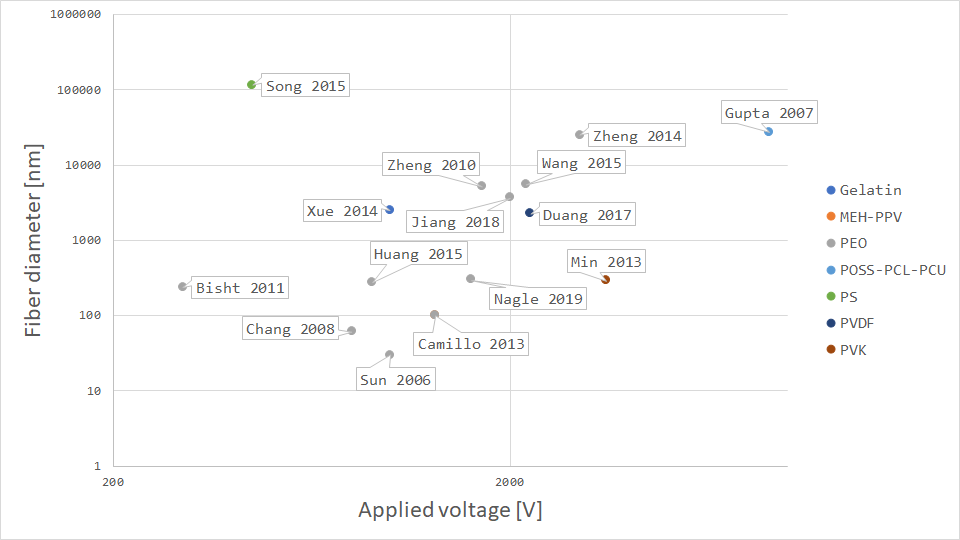
\includegraphics{images/e4441f91-c9b9-48f1-a3ed-5ec3e5033092-uplt_diametervolage.png}}{}
\makeatother 
\caption{{Applied volage vs. Fiber diameter}}
\label{f-59ed68f95344}
\end{figure*}
\egroup

\bgroup
\fixFloatSize{images/6198525c-7b44-494e-a092-206ecb3c8f9c-uweightdiameterplot.png}
\begin{figure*}[!htbp]
\centering \makeatletter\IfFileExists{images/6198525c-7b44-494e-a092-206ecb3c8f9c-uweightdiameterplot.png}{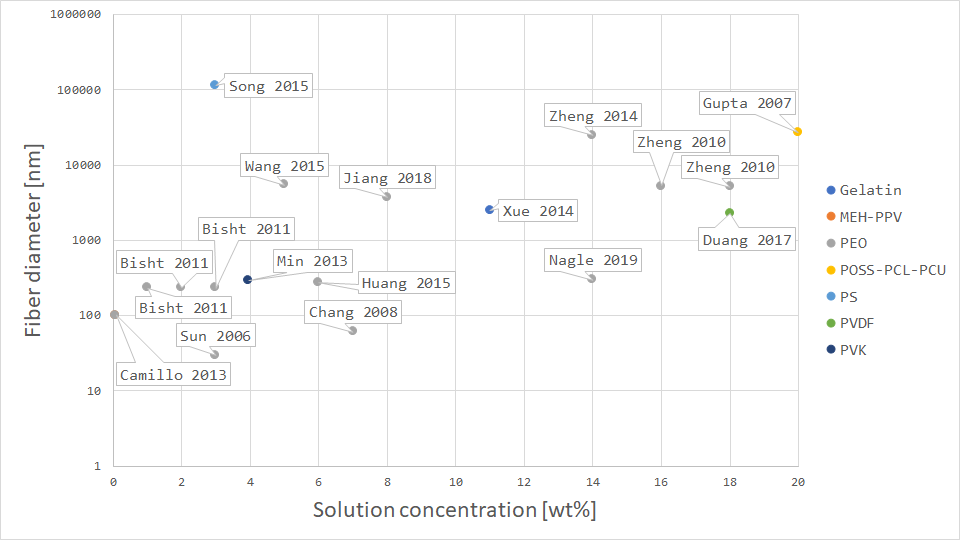
\includegraphics{images/6198525c-7b44-494e-a092-206ecb3c8f9c-uweightdiameterplot.png}}{}
\makeatother 
\caption{{Solution concentration vs. Fiber diameter}}
\label{f-0ba4df766d66}
\end{figure*}
\egroup

\bgroup
\fixFloatSize{images/fbd73f28-2c70-4a0a-be0b-f58ca8eab694-uweightconcentrationplot.png}
\begin{figure*}[!htbp]
\centering \makeatletter\IfFileExists{images/fbd73f28-2c70-4a0a-be0b-f58ca8eab694-uweightconcentrationplot.png}{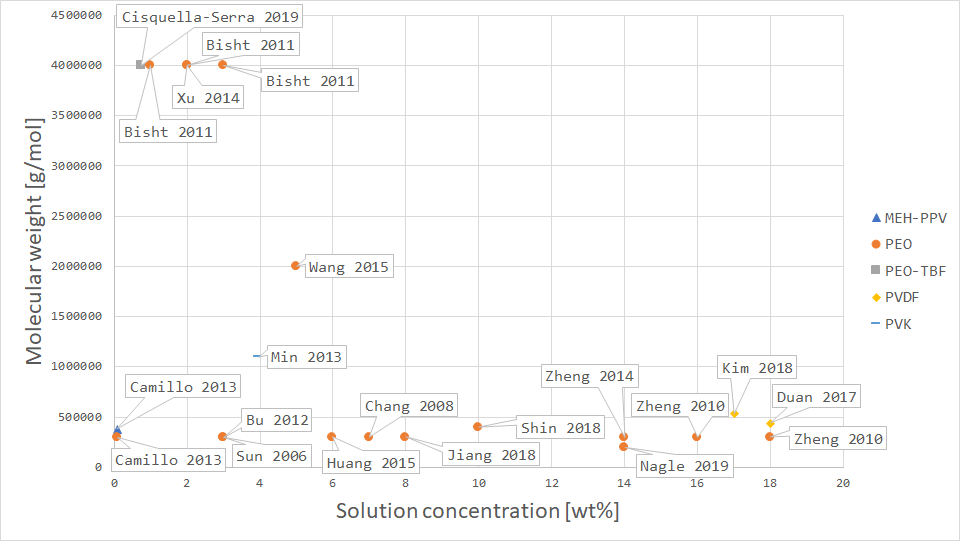
\includegraphics{images/fbd73f28-2c70-4a0a-be0b-f58ca8eab694-uweightconcentrationplot.png}}{}
\makeatother 
\caption{{Solution concentration vs. Molecular weight}}
\label{f-ab38f7e015f7}
\end{figure*}
\egroup
Lorem ipsum dolor sit amet, consectetur adipiscing elit, sed do eiusmod tempor incididunt ut labore et dolore magna aliqua. Ut enim ad minim veniam, quis nostrud exercitation ullamco laboris nisi ut aliquip ex ea commodo consequat. Duis aute irure dolor in reprehenderit in voluptate velit esse cillum dolore eu fugiat nulla pariatur. Excepteur sint occaecat cupidatat non proident, sunt in culpa qui officia deserunt mollit anim id est laborum.
    
\section{NFES Achievements \& Challenges}
Lorem ipsum dolor sit amet, consectetur adipiscing elit, sed do eiusmod tempor incididunt ut labore et dolore magna aliqua. Ut enim ad minim veniam, quis nostrud exercitation ullamco laboris nisi ut aliquip ex ea commodo consequat. Duis aute irure dolor in reprehenderit in voluptate velit esse cillum dolore eu fugiat nulla pariatur. Excepteur sint occaecat cupidatat non proident, sunt in culpa qui officia deserunt mollit anim id est laborum.
\apptocmd{\thebibliography}{\csname phantomsection\endcsname\addcontentsline{toc}{section}{\numberline{}\refname}}{}{}
    



\bibliographystyle{elsarticle-num}

\bibliography{\jobname}

\end{document}
